\documentclass[a4paper]{article}
\usepackage{amsmath}
\usepackage{amssymb}
\usepackage{bm}
\usepackage[UTF8]{ctex}
\usepackage{caption}
\usepackage{graphicx}
\usepackage{geometry}
\usepackage{tikz}
\usepackage{mmacells}

\setcounter{tocdepth}{4}
\setcounter{secnumdepth}{4}

\hypersetup{
colorlinks=true,
linkcolor=blue
}

\renewcommand\thesection{\Roman{section}}
\renewcommand\thesubsection{\arabic{subsection}}
\renewcommand\theparagraph{\alph{paragraph}}

\numberwithin{equation}{subsection}

\newtheorem{proof}{证明}
\newtheorem{theorem}{定理}
\newcommand{\mT}{\mathcal{T}}
\newcommand{\mC}{\mathcal{C}}
\newcommand{\mS}{\mathcal{S}}
\newcommand{\mU}{\mathcal{U}}
\newcommand{\mM}{\mathcal{M}}
\newcommand{\UT}{U_{T}}
\newcommand{\UC}{U_{C}}
\newcommand{\US}{U_{S}}

\geometry{left=2.0cm,right=2.0cm,top=2.0cm,bottom=2.0cm}

\begin{document}
\title{对称性分类}
\author{李成蹊}
\maketitle
\tableofcontents
\newpage
\section{对称性}
我们回顾不同的对称性是如何在费米系统中实现的。设$\{\psi_{I},\psi_I^\dagger\}_{I=1,\cdots,N}$是费米子产生湮灭算符的集合。我们这里为了简单起见假设我们已经正规化了格点系统,$I,J$是格点$i,j$和其他量子数(例如泡利自旋量子数$I=(i,\sigma)$)的结合指标。产生湮灭算符满足反对易关系$\{\psi_I,\psi_J^\dagger\}=\delta_{IJ}$.

我们现在考虑一个广义的无相互作用费米子系统,由二次量子化哈密顿$H$描述。对于非超导系统,$H$为
\begin{equation}
    \hat{H}=\psi_I^\dagger H^{IJ}\psi_J=\psi^\dagger H\psi
\end{equation}
其中,$N\times N$矩阵$H^{IJ}$是一次量子化哈密顿。在上述方程的右边,我们采用了爱因斯坦求和约定,最后一个等号是矩阵形式。(类似地,超导系统用Bogoliubov-de Gennes(BdG)哈密顿描述,我们用Nambu旋量而不是费米子算符,它的一次量子化形式还是在离散格点时的矩阵$H$)

根据对称表示理论,量子力学里任意的对称变换都可以表示为希尔伯特空间里的算符,这个算符要么是幺正的要么是反幺正的。我们从考虑一个幺正对称的例子开始,由一个算符集合$\{G_1,G_2,\cdots\}$描述,这个集合构成群。希尔伯特空间是它的表示空间$\{\mathcal{G}_1,\mathcal{G}_2,\cdots\}$,表示矩阵由这些算符作用在希尔伯特空间上得到。对于我们的目的,根据他们作用在费米子算符来引入对称变换是很方便的。也就是说,我们考虑一个线性变换
\begin{equation}
    \psi_I\rightarrow\psi_I':=\mathcal{U}\psi_I\mathcal{U}^{-1}=U_{I}^{J}\psi_J
\end{equation}
其中$\mathcal{U}$和$\psi_I,\psi_I^\dagger$是作用在费米子Fock空间的二次量子化算符。$U_I^J$是一堆数的几哈,实际上是表示矩阵,并不是二次量子化算符。更一般的可能是算符$\psi$和$\psi^\dagger$的混合幺正对称性。现在如果系统在$\mathcal{U}$下保持正则反对易关系和$\hat{H}$不变,则称这个系统是不变的。前一个条件意味着$U_I^J$是幺正矩阵,后一个条件可以得到$U^\dagger \hat{H}U=\hat{H}$

这里稍微证明一下上一段最后一句话

\begin{proof}
    \begin{equation}
        \begin{split}
            \psi_I\rightarrow\psi'_I&=\mathcal{U}\psi_I\mathcal{U}^{-1}=U_I^J\psi_J\\
            \psi_I^\dagger\rightarrow{\psi'}_I^\dagger&=(\mathcal{U}^{-1})^\dagger\psi_I^\dagger\mathcal{U}^\dagger=\psi_J^\dagger(U^{J}_{I})^*
        \end{split}
    \end{equation}
    要求$\{\psi'_I,{\psi'}_J^\dagger\}=\delta_{IJ}$保持不变则有
    \begin{equation}
        \{\psi'_I,{\psi'}_J^\dagger\}=\{U_I^{I'}\psi_{I'},\psi_{J'}(U_J^{J'})^*\}=U_I^{I'}(U_J^{I'})^*=\delta_{IJ}
    \end{equation}
    得证
\end{proof}
当幺正对称算符$\mathcal{U}$被作用在空间部分时(例如格点坐标$i,j$)被称为空间变换,当幺正对称算符$\mathcal{U}$被作用在自旋部分时(例如自旋坐标$\uparrow,\downarrow$)被称为非空间变换。当$\mathcal{U}$可以被分解为$\mathcal{U}=\prod_{i}\mathcal{U}_i$时(例如分别作用在不同的格点时),它不是空间变换,被称为在位。反幺正算符也有类似的定义。在这一节,我们关注于非空间对称,例如内部对称性,诸如TRS这种。空间对称在后面讨论。

值得注意,上述方程所考虑的这类幺正对称是一个全局对称性。正如我们在后面看到的,局域的对称性将会在SPT的探测中扮演至关重要的角色。
\subsection{时间反演对称}
我们现在考虑时间反演对称。时间反演是一个反幺正算符,作用在费米子产生湮灭算符上
\begin{equation}
    \mT\psi_I\mT^{-1}=(\UT)_I{}^J\psi_J,\quad \mT i\mT^{-1}=-i
\end{equation}
\begin{equation}
    \mT \psi_I^\dagger\mT^{-1}=\psi_J^\dagger(U_T^*)^J{}_{I}
\end{equation}
如果一个系统在时间反演下保持反对易关系不变,哈密顿满足$\mT \hat{H}\mT^{-1}=\hat{H}$,则称该系统时间反演不变。值得注意,如果厄米算符$O$由费米子算符构成,在$\mT$下保持不变,那么$\mT \hat{H}\mT^{-1}=\hat{H}$意味着
\begin{equation}
    \mT O(t)\mT^{-1}=\mT e^{i\hat{H}t}Oe^{-i\hat{H}t}\mT^{-1}=O(-t)
\end{equation}
在无相互作用系统里,$\mT \hat{H}\mT^{-1}=\hat{H}$可以推出
\begin{equation*}
    \begin{split}
        \mT \hat{H}\mT^{-1}&=\mT \psi_I^\dagger H^{IJ}\psi_J\mT^{-1}\\
        &=\mT\psi_I^\dagger\mT^{-1}\mT H^{IJ}\mT^{-1}\mT\psi_J\mT^{-1}\\
        &=\psi_{I'}^\dagger (U_T^*)^{I'}{}_{I}\mT H^{IJ}\mT^{-1}(U_T)_J{}^{J'}\psi_{J'}\\
        &=\psi_{I'}^\dagger(U_T^*)^{I'}{}_I (H^{IJ})^* (U_T)_{J}{}^{J'}\psi_{J'}
    \end{split}
\end{equation*}
\begin{equation}
    \hat{H}=\psi_I^\dagger H^{IJ}\psi_J=\mT H\mT^{-1}
\end{equation}
得到
\begin{equation}
    (U^{I'}{}_I)^*(H^{IJ})^*U_{J}{}^{J'}=H^{I'J'},\quad U_T^\dagger H^*U_T=H
\end{equation}
上式推导中,为了方便忽略了$U_T$的下标$T$. 我们得到
\begin{equation}
    \mT:U_T^\dagger H^* U_T=+H
\end{equation}
因为任何给定的哈密顿量都有许多偶然的,即非泛型的对称性,所以我们考虑以下对称是泛型的哈密顿量的整个参数族(即系综)。这种具有给定的一般对称集合的哈密顿集合称为对称类。我们现在让$H$跑遍所有可能的TRS对称类的单粒子哈密顿。用两边TRS条件,我们得到
\begin{equation}
    (U_T^\dagger)^* HU_T^*=H^*\Rightarrow U_T^\dagger (U_T^\dagger)^* HU_T^* U_T=U_T^\dagger H^* U_T=H
\end{equation}
我们得到
\begin{equation}
    (U_T^*U_T)^\dagger H(U_T^*U_T)=H
\end{equation}
因为一次量子化哈密顿$H$跑遍所有不可约表示空间,根据舒尔定理,$U_T^* U_T$是常数矩阵。
\begin{equation}
    U_T^*U_T=e^{i\alpha}\mathbf{1}
\end{equation}
因为$U_T$是幺正矩阵,可以得到
\begin{equation}
    U_T^*=e^{i\alpha}U_T^\dagger\Rightarrow (U_T)^T=e^{i\alpha}U_T
\end{equation}
因此我们得到$e^{2i\alpha}=1$,这推导出两个可能性$U_T^*U_T=\pm 1$. 这样用$T^2$作用在费米算符$\psi_I$仅仅会重新生成$\psi_I$,唯一不确定的是正负号
\begin{equation}
    \mT^2\psi_I\mT^{-2}=\mT (U_T)_I^J \psi_J\mT^{-1}=[(U_T)_I^J]^*(U_T)_J^K\psi_K=(U_T^*U_T\psi)_I=\pm\psi_I
\end{equation}
类似的对于由$n$个费米子产生湮灭算符组成的算符$O$来说,$\mT^2\hat{O}\mT^{-2}=(\pm 1)^n\hat{O}$. 总结来说,时间反演算符$\mT$满足
\begin{equation}
    \mT^2=(\pm 1)^{\hat{N}},\quad U_T^*U_T=\pm 1
\end{equation}
其中$N:=\sum_I\psi_I^\dagger\psi_I$是总费米子粒子数算符。特别地,当$U_T^*U_T=-1$,$\mT$平方对费米子数的宇称有下定义
\begin{equation}
    \mathcal{G}_f:=(-1)^{\hat{N}}
\end{equation}
对于有$\mT^2=-1$的系统,例如奇数个费米子系统满足$\mT^2=\mathcal{G}_f$,时间反演不变导致Kramers简并。
\subsection{粒子-空穴对称PHS}
粒子空穴对称$\mC$是一个混合费米子产生算符和湮灭算符的幺正变换:
\begin{equation}
    \mC\psi_I\mC^{-1}=(U_C^*)_I{}^J\psi_J^\dagger=\psi_J^\dagger(U_C^\dagger)^J{}_I=[(U_C)_I{}^J\psi_J]^\dagger
\end{equation}
\begin{equation}
    \mC\psi_I^\dagger\mC^{-1}=(U_C)_I{}^J\psi_J
\end{equation}
$\mC$通常也被称为电荷共轭对称,因为在粒子数守恒的系统里,它翻转$U(1)$规范的荷$\mC Q\mC^{-1}=-Q$,其中$Q=N-N/2$,$N/2$是轨道数的一半,例如单粒子希尔伯特空间维数的一半。在$\mC$变换下,正则反对易关系保持不变的要求,这让我们看到$U_C$是一个幺正矩阵。在无相互作用哈密顿$\hat{H}$中,PHS导致
\begin{equation}
    \begin{split}
        \hat{H}&=\mC\hat{H}\mC^{-1}\\
        &=\mC\psi_I^\dagger H^{IJ} \psi_J \mC^{-1}\\
        &=\mC\psi_I^\dagger\mC^{-1}\mC H^{IJ}\mC^{-1}\mC\psi_J\mC^{-1}\\
        &=(U_C)_I{}^{I'}\psi_{I'}\mC H^{IJ}\mC^{-1} (U_C^*)_J{}^{J'}\psi_{J'}^\dagger\\
        &=(U_C)_I{}^{I'}(U_C^*)_J{}^{J'}\psi_{I'}H^{IJ}\psi_{J'}^\dagger\\
        &=-(U_C)_I{}^{I'}(U_C^*)_J{}^{J'}\psi_{J'}^\dagger H^{IJ}\psi_{I'}+(U_C)_I{}^{I'}(U_C^*)_J^{J'}H^{IJ}\delta_{I'J'}\\
        &=-\psi_{J'}^\dagger(U_C^\dagger)^{J'}{}_JH^{IJ}(U_C)_I^{}{I'}\psi_{I'}+Tr(H)\\
        &=-\psi^\dagger(U_C^\dagger H^TU_C)\psi+Tr(H)=\psi^\dagger H\psi
    \end{split}
\end{equation}
这意味着
\begin{equation}
    \mC: U_C^\dagger H^T U_C=-H
\end{equation}
观察上式得到$Tr(H)=H^{II}=0$. 因为$H$是厄米的,单粒子哈密顿的PHS条件可以写成$-U_C^\dagger H^*U_C=H$. 观察PHS条件表明当$\mC$作用在单粒子希尔伯特空间时,$\mC$不是一个幺正对称性,而是哈密顿模去幺正转动的实现条件。通过重复与TRS相同的操作,我们可以看到有两类PH变换
\begin{equation}
    U_C^\dagger H^T U_C=-H\Rightarrow U_C^THU_C^*=-H^T
\end{equation}
\begin{equation}
    U_C^\dagger U_C^THU_C^*U_C=-U_C^\dagger H^TU_C=H
\end{equation}
$H$跑遍所有的不可约表示空间,可以得知$U_C^*U_C=e^{i\alpha}\mathbf{1}$. 这意味着$U_C=e^{i\alpha}U_C^T=e^{2i\alpha}U_C$, 所以$U_C^*U_C=\pm 1$. 同样的计算$\mC^2\psi_I\mC^{-2}$
\begin{equation}
    \mC^2\psi_I\mC^{-2}=\mC (U_C^*)_I{}^J\psi_J^\dagger\mC^{-1}=(U_C^*)_I{}^JU_J{}^K\psi_K=(\pm 1)\psi_I
\end{equation}
总结而言
\begin{equation}
    \mC^2=(\pm 1)^{\hat{N}},\quad U_C^*U_C=\pm 1
\end{equation}
在PHS系统里,$\mC \hat{H}\mC^{-1}=\hat{H}$,对于每一个能量本征态$|\alpha\rangle$的PH反演对也是能量本征态,因为$\hat{H}\mC|\alpha\rangle=\mC \hat{H}\mC^{-1}\mC|\alpha\rangle=E_\alpha\mC|\alpha\rangle$. 类似的,对于单粒子哈密顿,对于每一个对应能量$\varepsilon^A$哈密顿$H$的本征函数$u^A$,$H^{IJ}u^A_J=\varepsilon^A u_{I}^{A}$,有PH反演对$U_C^\dagger (u^A)^*$也是本征函数,但是能量为$-\varepsilon^A$,因为$HU_C^\dagger(u^A)^*=-U_C^\dagger H^*U_CU_C^\dagger (u^A)^*=-\varepsilon^AU_C^\dagger(u^A)^*$
\begin{equation}
    \begin{split}
        Hu^A&=\varepsilon^Au^A,\quad H^*(u^A)^*=\varepsilon^A (u^A)^*,\quad H^T=H^*
    \end{split}
\end{equation}
\begin{equation}
    U_C^\dagger H^TU_C=-H\Rightarrow U_C^\dagger H^T=-HU_C^\dagger\Rightarrow-H\Rightarrow U_C^\dagger H^*=-HU_C^\dagger
\end{equation}
\begin{equation}
    U_C^\dagger H^*(u^A)^*=-HU_C^\dagger (u^A)^*=\varepsilon^A U_C^\dagger(u^A)^*\Rightarrow HU_C^\dagger (u^A)^*=-\varepsilon^AU_C^\dagger(u^A)^*
\end{equation}
作为一个PH对称系统的例子,我们研究定义在双粒子晶格上的Hubbard模型
\begin{equation}
    \hat{H}=\sum_{ij}^{i\neq j}\sum_{\sigma}t_{ij}c_{i\sigma}^\dagger c_{j\sigma}-\mu\sum_{i}\sum_{\sigma}n_{i\sigma}+U\sum_{i}n_{i\uparrow}n_{i\downarrow}
\end{equation}
其中$c_{i\sigma}^\dagger$是电子在格点$i$自旋为$\sigma=\uparrow,\downarrow$的产生算符,$n=c_{\sigma}c_{i\sigma}$. 这里$t_{ij}=t_{ji}^*$,$mu$和$U$表示Hopping矩阵元,化学势和相互作用强度。现在考虑如下的PH变换
\begin{equation}
    \mC c_{i\sigma}\mC^{-1}=(-1)^{i}c_{i\sigma}^\dagger,\quad \mC c_{i\sigma}^\dagger\mC^{-1}=(-1)^{i}c_{i\sigma}
\end{equation}
其中$(-1)^i$表示位置$i$的正负号,代表不同子格。当$\mu=U/2$并且$t_{ij}$连接子格相同(不同)子格格点时纯虚数(实数)时,上述哈密顿在$\mC$变换下不变。
\begin{equation*}
    \hat{H}_{int}=-\mu\sum_i\sum_\sigma n_{i\sigma}+U\sum_{i}n_{i\uparrow}n_{i\downarrow}
\end{equation*}
\begin{equation*}
    \begin{split}
        \hat{H}_{int}\rightarrow\mC\hat{H}_{int}\mC^{-1}&=-\mu\sum_{i\sigma}c_{i\sigma}c_{i\sigma}^\dagger+U\sum_{i}c_{i\uparrow}c_{i\uparrow}^\dagger c_{i\downarrow}c_{i\downarrow}^\dagger\\
        &=\mu\sum_{i\sigma}(c_{i\sigma}^\dagger c_{i\sigma}-1)+U\sum_{i}(1-c_{i\uparrow}^\dagger c_{i\uparrow})(1-c_{i\downarrow}^\dagger c_{i\downarrow})\\
        &=\mu\sum_{i\sigma}n_{i\sigma}-2\mu L+U\sum_{i}n_{i\uparrow}n_{i\downarrow}-U\sum_{i}(n_{i\uparrow}+n_{i\downarrow})+UL\\
        &=(\mu-U)\sum_{i\sigma}n_{i\sigma}+U\sum_{i}n_{i\uparrow}n_{i\downarrow}-(2\mu-U)L
    \end{split}
\end{equation*}
所以$\mu=\frac{U}{2}$时,Hubbard模型满足PHS.
\subsection{手征对称性/子格对称性}
把TRS与PHS结合到一起可以得到第三种对称性,叫做手征对称性。也就是说,可以有这种情况,$\mT,\mS$都是破缺的,但他们的组合却是对称的
\begin{equation}
    \mS=\mT\cdot\mC
\end{equation}
手征对称$\mS$作用在费米子算符上为
\begin{equation}
    \mS \psi_I\mS=(U_CU_T)_{I}{}^J\psi_J^\dagger
\end{equation}
从$\mS\hat{H}\mS^{-1}=\hat{H}$可以推出哈密顿二次型在$\mS$变换下的描述为
\begin{equation}
    \mS:U_S^\dagger HU_S=-H,\quad U_S=U_C^*U_T^*
\end{equation}
值得注意,上式可以得到$Tr(H)=0$. 相同的手段我们可以看到
\begin{equation}
    (U_S^2)^\dagger HU_S^2=H\Rightarrow HU_S^2=U_S^2 H
\end{equation}
所以$U_S^2-e^{i\alpha}\mathbf{1}$. 这样可以重新定义$U_S\rightarrow e^{i\alpha/2}U_S$,单粒子哈密顿手征对称条件化简为
\begin{equation}
    \mS:\{H,U_S\}=0,\quad U_S^2=U_S^\dagger U_S=1
\end{equation}
从这里可以看出,手征算符的本征值是$\pm 1$. 除此之外,还可以提出一个条件$Tr(U_S)=0$(然而这并不是必须的)。手征对称产生了单粒子哈密顿的对称谱:如果$|u\rangle$是哈密顿$H$能量为$\varepsilon$的本征态,那么$U_S|u\rangle$也是它的本征态,本征值对应为$-\varepsilon$. 在这个基构成的空间里,$U_S$是对角的,单粒子哈密顿$H$是反对角的,
\begin{equation}
    H=\begin{pmatrix}
        0&D\\
        D^\dagger&0
    \end{pmatrix}
\end{equation}
$D$是$N_A\times N_B$的方片矩阵,$N_A+N_B=N$.

作为一个粒子,我们考虑紧束缚无自旋费米子哈密顿
\begin{equation}
    \hat{H}=\sum_{m,n}t_{mn}c_m^\dagger c_n,\quad t_{m,n}=t_{nm}^*\in\mathbf{C}
\end{equation}
为了构造手征对称,我们结合PH对称和TR对称,这定义成$\mT c_m\mT^{-1}=c_m,\mT i\mT^{-1}=-i$. 这导致对称条件$\mS c_m\mS^{-1}=(-1)^m c_m^\dagger, \mS i\mS^{-1}=-i$. 当$t_{mn}$仅仅是连接不同子格之间的hopping时,$\hat{H}$是不变的。观察这个例子
\begin{equation}
    Tr(U_S)=\sum_{n}\langle n|U_S|n\rangle=\sum_{n\in N_A}\langle n|n\rangle-\sum_{n\in N_B}\langle n|n\rangle=N_A-N_B,\quad U_S|n\rangle=\begin{cases}
        |n\rangle\quad &n\in N_A\\
        -|n\rangle\quad &n\in N_B
    \end{cases}
\end{equation}
其中$N_A,N_B$分别是子格$A,B$格点数

除了上述双粒子Hopping模型,手征对称性也在玻色系统里实现了。

\subsection{BdG系统}
具有PHS和手性对称性的系统的重要例子是BdG哈密顿量,我们将在本节讨论。这些例子说明了物理上不同的多体对称条件可能导致单粒子哈密顿约束有相同集合
\subsubsection{Class D}
BdG哈密顿有Nambu旋量定义
\begin{equation}
    \Psi=\begin{pmatrix}
        \psi_1\\
        \vdots\\
        \psi_N\\
        \psi_1^\dagger\\
        \vdots\\
        \psi_N^\dagger
    \end{pmatrix},\quad
        \Psi^\dagger=\begin{pmatrix}
            \psi_1^\dagger&\cdots&\psi_N^\dagger&\psi_1&\cdots&\psi_N
        \end{pmatrix}
\end{equation}
他们满足正则反对易关系$\{\Psi_A,\Psi_B\}=\delta_{AB},\{A,B=1,2,\cdots,2N\}$. 记住$\Psi$和$\Psi^\dagger$不是独立的很关键,但是他们之间有联系
\begin{equation}\label{BdG relation}
    (\tau_1\Psi)^T=\Psi^\dagger,\quad (\Psi^\dagger\tau_1)^T=\Psi
\end{equation}
其中泡利矩阵$\tau_1$作用在Nambu空间上。实际上是$\tau_1=\sigma_x\otimes \mathbf{I}_N$. 利用Nambu旋量,BdG哈密顿$\hat{H}$可以写成
\begin{equation}
    \hat{H}=\frac{1}{2}\Psi_A^\dagger H^{AB}\Psi_B=\frac{1}{2}\Psi^\dagger H\Psi
\end{equation}
\begin{equation}
    \hat{H}=\psi_A^\dagger h^{AB}\psi_B=\frac{1}{2}\psi_A^\dagger h^{AB}\psi_B+\frac{1}{2}(\delta_{AB}h^{AB}-\psi_A (h^T)^{AB}\psi_B^\dagger)=\frac{1}{2}\Psi_A^\dagger H^{AB}\Psi_{B}+\frac{1}{2}Tr(h)
\end{equation}
\begin{equation}
    H=\begin{pmatrix}
        h&0\\
        0&-h^T
    \end{pmatrix}
\end{equation}
因为$\Psi$和$\Psi^\dagger$不是独立的,单粒子哈密顿$H$必须满足一个约束。利用方程\eqref{BdG relation},我们可以得到
\begin{equation}
    \begin{split}
        \hat{H}&=\frac{1}{2}(\tau_1\Psi)^TH(\Psi^\dagger\tau_1)^T=\frac{1}{2}[(\tau_1\Psi)^T]_{A}H^{AB}[(\Psi^\dagger \tau_1)^T]_{B}\\
        &=\frac{1}{2}[\Psi^T\tau_1]_AH^{AB}[\tau_1\Psi^*]_B=\frac{1}{2}(\Psi^T)_{A'}(\tau_1)_{A'A}H^{AB}(\tau_1)_{BB'}\Psi^*_{B'}\\
        &=-\frac{1}{2}\Psi_B^*(\tau_1)_{A'A}H^{AB}(\tau_1)_{BB'}(\Psi^T)_{A'}+\frac{1}{2}(\tau_1)_{A'A}H^{AB}(\tau_1)_{BB'}\delta_{A'B'}\\
        &=-\frac{1}{2}\Psi^\dagger(\tau_1 H\tau_1)^T\Psi+\frac{1}{2}Tr)(\tau_1H\tau_1)
    \end{split}
\end{equation}
所以有
\begin{equation}
    \tau_1H^T\tau_1=-H
\end{equation}
这样,每一个单粒子BdG哈密顿满足PHS。然而,上述条件并不是由于外加的对称性产生的,而是由于BdG哈密顿内置的来自费米统计的特性。因此,在BdG系统中$\tau_1 H^T\tau_1=-H$应该被叫做粒子-空穴守恒,或者费米子守恒,并不是一个对称性。由于方程$\tau_1 H^T\tau_1=-H$,任何BdG哈密顿都可以写成
\begin{equation}
    H=\begin{pmatrix}
        \xi&\Delta\\
        -\Delta^*&-\xi^T
    \end{pmatrix},\quad \xi=\xi^\dagger,\quad \Delta^T=-\Delta
\end{equation}
其中$\xi$表示正常部分,$\Delta$表示反正部分(比如配对项),

BdG哈密顿可以认为是马约拉纳费米子单粒子哈密顿。BdG哈密顿的马约拉纳表示由下得到
\begin{equation}
    \begin{pmatrix}
        \lambda_I\\
        \lambda_{I+N}
    \end{pmatrix}=\begin{pmatrix}
        \psi_I+\psi_I^\dagger\\
        i(\psi_I-\psi_I^\dagger)
    \end{pmatrix}
\end{equation}
\begin{equation}
    \begin{pmatrix}
        \lambda_1\\
        \vdots\\
        \lambda_N\\
        \lambda_{N+1}^\dagger\\
        \vdots\\
        \lambda_{2N}^\dagger
    \end{pmatrix}=\begin{pmatrix}
        I_N&I_N\\
        iI_N&-iI_N
    \end{pmatrix}\begin{pmatrix}
        \psi_1\\
        \vdots\\
        \psi_N\\
        \psi_1^\dagger\\
        \vdots\\
        \psi_N^\dagger
    \end{pmatrix}\Rightarrow \lambda=\Omega\Psi
\end{equation}
马约拉纳费米满足
\begin{equation}
    \{\lambda_A,\lambda_B\}=2\delta_{AB},\quad\lambda_A^\dagger=\lambda_A,\quad (A,B=1,2,\cdots,2N)
\end{equation}
\begin{enumerate}
    \item $\{\lambda_A,\lambda\}=\{\psi_A+\psi_A,\psi_B+\psi_B^\dagger\}=\{\psi_A,\psi_B^\dagger\}+\{\psi_A^\dagger,\psi_B\}=2\delta_{AB}$
    \item $\{\lambda_A,\lambda_B\}=\{\psi_A+\psi_A^\dagger,i(\psi_B-\psi_B^\dagger)\}=-i\{\psi_A,\psi_B^\dagger\}+i\{\psi_A^\dagger,\psi_B\}=0$
    \item $\{i(\psi_A-\psi_A^\dagger),i(\psi_B-\psi_B^\dagger)\}=\{\psi_A,\psi_B^\dagger\}+\{\psi_A^\dagger,\psi_B\}=2\delta_{AB}$
\end{enumerate}
在这个马约拉纳基底里,BdG哈密顿可以写成
\begin{equation}
    \hat{H}=\Psi^\dagger H\Psi=\Psi^\dagger \Omega^\dagger\Omega H\Omega^\dagger \Omega \Psi=i\lambda^\dagger X\lambda
\end{equation}
其中
\begin{equation}
    iX=\Omega H \Omega^\dagger=\begin{pmatrix}
        \frac{1}{2}&-\frac{i}{2}\\
        \frac{1}{2}&\frac{i}{2}
    \end{pmatrix}\begin{pmatrix}
        \xi&\Delta\\
        -\Delta^*&-\xi^T
    \end{pmatrix}\begin{pmatrix}
        1&1\\
        i&-i
    \end{pmatrix}=\begin{pmatrix}
        R_-+S_-&-i(R_+-S_+)\\
        i(R_++S_+)&R_--S_-
    \end{pmatrix},\quad X^T=-X
\end{equation}
\begin{equation}
    \begin{cases}
        R_+=\xi+\xi^T,&\quad R_+^T=R_+,\quad R_+^*=R_+\\
        R_-=\xi-\xi^T,&\quad R_-^T=-R_-,\quad R_-^*=-R_-\\
        S_+=\Delta+\Delta^*,&\quad S_+^T=-S_+,\quad S_+^*=S_+\\
        S_-=\Delta-\Delta^*,&\quad S_-^T=-S_-,\quad S_-^*=-S_-
    \end{cases}
\end{equation}
我们注意实斜对称阵$X$可以通过正交变换变成块对角矩阵。
\begin{equation}
    X=O\Sigma O^T,\quad\Sigma=\begin{pmatrix}
        0&\varepsilon_1\\
        -\varepsilon_1&0\\
        &&\ldots\\
        &&&0&\varepsilon_N\\
        &&&-\varepsilon_N&0
    \end{pmatrix}
\end{equation}
其中$O$是正交矩阵,$\varepsilon_I\geq0$. 转动基底$\xi:=O^T\lambda$,哈密顿有形式$\hat{H}=i\xi^T\Sigma\xi=2\sum_{I=1}^N\varepsilon_I\xi_{2I-1}\xi_{2I}$

虽然用马约拉纳算符重写BdG哈密顿量总是可能的,但马约拉纳算符是哈密顿量的本征态是相当罕见的。也就是说,未配对或孤立的Majorana零能本征态在BdG系统中非常罕见,只出现在特殊情况下。此外,我们注意到,一般来说,没有一种自然的方法可以将给定的马约拉纳哈密顿量改写为BdG哈密顿量,因为一般来说,没有任何自然的方法可以说明如何从给定的马约拉纳算符集合中形成复费米子算符。(要定义好这样一个公式,一个必要条件是马约拉纳哈密顿量必须是一个偶维矩阵。)

综上所述,单粒子BdG哈密顿具有PH守恒的特征。满足PHS的哈密顿集合称为Class D。通过施加各种对称,BdG哈密顿可以实现其他五个对称Class:DIII, A, AIII, C,和CI,我们将在下面讨论。
\subsubsection{Class DIII}
我们从研究满足$\mT^2=\mathcal{G}_f$的TRS下BdG哈密顿的约束形式。出于这个目的,我们把费米子算符标记自旋,例如我们设$\psi_I=\psi_{I\sigma}$. 我们引入TRS条件
\begin{equation}
    \mT\psi_{I\sigma}\mT^{-1}=(i\sigma_2)_{\sigma\sigma'}\psi_{I\sigma'}
\end{equation}
其中$\sigma_2$是作用在自旋空间的泡利矩阵。BdG哈密顿满足
\begin{equation}
    \tau_1 H^T \tau_1=-H,\quad\sigma_2 H^*\sigma_2=H
\end{equation}
值得注意,上面的$\tau_1$作用于Nambu空间,$\sigma_2$作用于自旋空间。正如我们之前讨论的,PH守恒荷TRS可以结合成手征对称性$\tau_1\sigma_2 H\sigma_2\tau_1=-H$. 观察在这个手征对称性的实现中$TrU_S=0$. 满足上述对称性条件的哈密顿集合叫做Class DIII.(如果把条件$\mT^2=\mathcal{G}_f$替换为$\mT^2=1$将会导致一个不同的Class,称为BDI)

\subsubsection{Class A和AIII}
接下来我们讨论有在自旋空间中绕$S_z$轴$U(1)$自旋转动对称的BdG系统。这个对称性允许我们重新调整BdG哈密顿到一个约化的形式
\begin{equation}\label{class a}
    \hat{H}=\Psi_A^\dagger H^{AB}\Psi_B
\end{equation}
其中$H$是$2N$维没有约束的矩阵
\begin{equation}\label{spinor}
    \Psi^\dagger=\begin{pmatrix}
        \psi_{I\uparrow}^\dagger&\psi_{I\downarrow}
    \end{pmatrix},\quad \Psi=\begin{pmatrix}
        \psi_{I\uparrow}\\
        \psi_{I\downarrow}^\dagger
    \end{pmatrix}
\end{equation}
因为$H$没有约束,这个哈密顿属于Class A.

这个系统满足绕$z$轴的$U(1)$转动$\mU_{S_z}^\phi=e^{-i(\frac{\phi}{2})\sigma_z}$. 这个转动作用在基本二分量旋量上为
\begin{equation}
    \mU_{S_z}^{\phi}=e^{-i\frac{\phi}{2}\sigma_z}\begin{pmatrix}
        \psi_\uparrow\\
        \psi_\downarrow
    \end{pmatrix}=\begin{pmatrix}
        e^{-i\frac{\phi}{2}}\\
        &e^{i\frac{\phi}{2}}
    \end{pmatrix}\begin{pmatrix}
        \psi_\uparrow\\
        \psi_\downarrow
    \end{pmatrix}
\end{equation}
所以我们有在$U(1)$转动变换下:
\begin{equation}
    \begin{cases}
        \psi_\uparrow\rightarrow e^{-i\frac{\phi}{2}}\psi_\uparrow\\
        \psi_\downarrow\rightarrow e^{i\frac{\phi}{2}}\psi_\downarrow\\
        \psi_\uparrow^\dagger\rightarrow e^{i\frac{\phi}{2}}\psi_\uparrow^\dagger\\
        \psi_\downarrow^\dagger\rightarrow e^{-i\frac{\phi}{2}}\psi_\downarrow^\dagger
    \end{cases}\Rightarrow\Psi\rightarrow\mU_{S_z}^\phi\Psi\mU_{S_z}^{-\phi}= e^{-i\frac{\phi}{2}}\Psi
\end{equation}
满足绕$z$轴$U(1)$转动对称哈密顿为:
\begin{equation}
    \hat{H}=\mU_{S_z}^{\phi}\hat{H}\mU_{S_z}^{-\phi}=\mU_{S_z}^{\phi}\Psi^\dagger\mU_{S_z}^{-\phi}\mU_{S_z}^{\phi}H\mU_{S_z}^{-\phi}\mU_{S_z}^{\phi}\Psi\mU_{S_z}^{-\phi}=\Psi(\mU_{S_z}^{\phi}H\mU_{S_z}^{-\phi})\Psi
\end{equation}
绕$z$轴$U(1)$转动对称条件为
\begin{equation}
    S_zHS_z^{-1}=H
\end{equation}
因为$\Psi$和$\Psi^\dagger$是完全独立的算符,把费米算符做$\psi_{\downarrow}^\dagger\rightarrow \psi_\downarrow,\psi_{\downarrow}\rightarrow\psi_\downarrow^\dagger$的替换是可能的。通过这样的替换,BdG哈密顿可以转化为一个正常的粒子数守恒费米子系统:
\begin{equation}
    \Psi^\dagger\rightarrow\begin{pmatrix}
        \psi_\uparrow^\dagger&\psi_\downarrow^\dagger
    \end{pmatrix},\quad \Psi\rightarrow\begin{pmatrix}
        \psi_\uparrow\\
        \psi_\downarrow
    \end{pmatrix},\quad [\hat{H},\hat{N}]=0,\quad \hat{N}=\psi_\uparrow^\dagger\psi_\uparrow+\psi_\downarrow^\dagger\psi_\downarrow
\end{equation}
在这个过程里BdG系统的$U(1)$自旋旋转对称性变成一个虚拟的$U(1)$规范荷对称。
\begin{equation}
    \Psi=\begin{pmatrix}
        \psi_\uparrow\\
        \psi_\downarrow^\dagger
    \end{pmatrix}\rightarrow e^{-i\frac{\phi}{2}}\begin{pmatrix}
        \psi_\uparrow\\
        \psi_\downarrow^\dagger
    \end{pmatrix}=e^{-i\frac{\phi}{2}}\Psi\quad\text{(绕$S_z$轴自旋旋转对称)}
\end{equation}
\begin{equation}
    \Psi=\begin{pmatrix}
        \psi_\uparrow\\
        \psi_\downarrow
    \end{pmatrix}\rightarrow e^{-i\frac{\phi}{2}}\begin{pmatrix}
        \psi_\uparrow\\
        \psi_\downarrow
    \end{pmatrix}=e^{-i\frac{\phi}{2}}\Psi\quad\text{(替换后变成粒子数守恒系统的$U(1)$规范对称)}
\end{equation}
我们现在对原哈密顿添加$TRS$,作用在$\Psi$为
\begin{equation}
    \mT\Psi \mT^{-1}=\mT\begin{pmatrix}
        \psi_\uparrow\\
        \psi_\downarrow^\dagger
    \end{pmatrix}\mT^{-1}=\begin{pmatrix}
        \psi_\downarrow\\
        -\psi_\uparrow^\dagger
    \end{pmatrix}=i\rho_2(\Psi^\dagger)^T=:\Psi^c
\end{equation}
其中$\rho_{1,2,3}$表示作用在旋量\eqref{spinor}的粒子-空穴上和自旋分量上的泡利矩阵。观察这个,如果我们令$\psi_\uparrow^\dagger\rightarrow\psi_\uparrow$,那么$\mT$在上述变换中表现得像$\mT$和$\mC$的组合,也就是手征对称。
\begin{equation}
    \begin{cases}
        \psi_\uparrow^\dagger\rightarrow\psi_\uparrow\\
        \psi_\uparrow\rightarrow\psi_\uparrow^\dagger
    \end{cases},\quad \mT \begin{pmatrix}
        \psi_\uparrow^\dagger\\
        \psi_\downarrow^\dagger
    \end{pmatrix}\mT^{-1}=\begin{pmatrix}
        \psi_\downarrow\\
        -\psi_\uparrow
    \end{pmatrix},\quad\text{(这里的$\mT$并不表示时间反演,表示替换后的对称性)}
\end{equation}
手征对称性$\mT\mC$和$U(1)$荷$Q$在粒子数守恒系统里$(\mT\mC)Q(\mT\mC)^{-1}=Q$的关系同构于$TRS$和$S_z$在$BdG$系统里$S_z$守恒的关系$\mT S_z\mT^{-1}=S_z$. 也就是说,通过将式\eqref{class a}重新解释为粒子数守恒系统,TRS变成了手征对称。

满足手征对称的哈密顿集合叫做Class AIII. 因此,具有$S_z$守恒荷$TRS$的BdG系统属于Class A和AIII.
\subsubsection{Class C和Class CI}
我们现在研究由于$SU(2)$自旋旋转对称而不是$S_z$守恒的约束。一个绕轴$\mathbf{n}$旋转$\phi$的自旋转动$\mU_{\mathbf{n}}^\phi$作用在二分量旋量上为
\begin{equation}
    \begin{pmatrix}
        \psi_\uparrow\\
        \psi_\downarrow\\
    \end{pmatrix}\rightarrow\mU_{\mathbf{n}}^\phi\begin{pmatrix}
        \psi_\uparrow\\
        \psi_\downarrow
    \end{pmatrix},\quad \mU_{\mathbf{n}}^{\phi}=e^{-i\frac{\phi}{2}\mathbf{\sigma}\cdot\mathbf{n}}
\end{equation}
绕$S_x,S_y$方向的转动$\phi$的变换为
\begin{equation}
    \mU_{S_x}^\phi\begin{pmatrix}
        \psi_{\uparrow}\\
        \psi_{\downarrow}
    \end{pmatrix}=\begin{pmatrix}
        \cos\frac{\phi}{2}&-i\sin\frac{\phi}{2}\\
        -i\sin\frac{\phi}{2}&\cos\frac{\phi}{2}
    \end{pmatrix}\begin{pmatrix}
        \phi_\uparrow\\
        \phi_\downarrow
    \end{pmatrix}=\begin{pmatrix}
        \cos\frac{\phi}{2}\psi_\uparrow-i\sin\frac{\phi}{2}\psi_\downarrow\\
        -i\sin\frac{\phi}{2}\psi_\uparrow+\cos\frac{\phi}{2}\psi_\downarrow
    \end{pmatrix}
\end{equation}
\begin{equation}
    \mU_{S_y}^\phi\begin{pmatrix}
        \phi_\uparrow\\
        \phi_\downarrow
    \end{pmatrix}=\begin{pmatrix}
        \cos\frac{\phi}{2}&-\sin\frac{\phi}{2}\\
        \sin\frac{\phi}{2}&\cos\frac{\phi}{2}
    \end{pmatrix}\begin{pmatrix}
        \phi_\uparrow\\
        \phi_\downarrow
    \end{pmatrix}=\begin{pmatrix}
        \cos\frac{\phi}{2}\psi_\uparrow-\sin\frac{\phi}{2}\psi_\downarrow\\
        \sin\frac{\phi}{2}\psi_\uparrow+\cos\frac{\phi}{2}\psi_\downarrow
    \end{pmatrix}
\end{equation}
我们有SU(2)下,各个费米子算符变换形式
\begin{equation}
    \begin{split}
        &\mU_{S_x}^\phi\psi_\uparrow\mU_{S_x}^{-\phi}=\cos\frac{\phi}{2}\psi_\uparrow-i\sin\frac{\phi}{2}\psi_\downarrow\\
        &\mU_{S_x}^\phi\psi_\downarrow\mU_{S_x}^{-\phi}=-i\sin\frac{\phi}{2}\psi_\uparrow+\cos\frac{\phi}{2}\psi_\downarrow\\
        &\mU_{S_x}^\phi\psi_\uparrow^\dagger\mU_{S_x}^{-\phi}=\cos\frac{\phi}{2}\psi_\uparrow+i\sin\frac{\phi}{2}\psi_\downarrow\\
        &\mU_{S_x}^\phi\psi_\downarrow^\dagger\mU_{S_x}^{-\phi}=i\sin\frac{\phi}{2}\psi_\uparrow+\cos\frac{\phi}{2}\psi_\downarrow
    \end{split}
\end{equation}
\begin{equation}
    \begin{split}
        &\mU_{S_y}^\phi\psi_\uparrow\mU_{S_y}^{-\phi}=\cos\frac{\phi}{2}\psi_\uparrow-\sin\frac{\phi}{2}\psi_\downarrow\\
        &\mU_{S_y}^\phi\psi_\downarrow\mU_{S_y}^{-\phi}=\sin\frac{\phi}{2}\psi_\uparrow+\cos\frac{\phi}{2}\psi_\downarrow\\
        &\mU_{S_y}^\phi\psi_\uparrow^\dagger\mU_{S_y}^{-\phi}=\cos\frac{\phi}{2}\psi_\uparrow-\sin\frac{\phi}{2}\psi_\downarrow\\
        &\mU_{S_y}^\phi\psi_\downarrow^\dagger\mU_{S_y}^{-\phi}=\sin\frac{\phi}{2}\psi_\uparrow+\cos\frac{\phi}{2}\psi_\downarrow
    \end{split}
\end{equation}
所以我们有
\begin{equation}
    \mU_{S_x}^\phi\Psi\mU_{S_x}^{-\phi}=\mU_{S_x}^\phi\begin{pmatrix}
        \psi_\uparrow\\
        \psi_\downarrow^\dagger
    \end{pmatrix}\mU_{S_x}^{-\phi}=\begin{pmatrix}
        \cos\frac{\phi}{2}\psi_\uparrow-i\sin\frac{\phi}{2}\psi_\downarrow\\
        i\sin\frac{\phi}{2}\psi_\uparrow^\dagger+\cos\frac{\phi}{2}\psi_\downarrow^\dagger
    \end{pmatrix}=\cos\frac{\phi}{2}\Psi-i\sin\frac{\phi}{2}\Psi^c
\end{equation}
\begin{equation}
    \mU_{S_y}^\phi\Psi\mU_{S_y}^{-\phi}=\mU_{S_y}^\phi\begin{pmatrix}
        \psi_\uparrow\\
        \psi_\downarrow^\dagger
    \end{pmatrix}\mU_{S_y}^{-\phi}=\begin{pmatrix}
        \cos\frac{\phi}{2}\psi_\uparrow-\sin\frac{\phi}{2}\psi_\downarrow\\
        \sin\frac{\phi}{2}\psi_\uparrow^\dagger+\cos\frac{\phi}{2}\psi_\downarrow^\dagger
    \end{pmatrix}=\cos\frac{\phi}{2}\Psi-\sin\frac{\phi}{2}\Psi^c
\end{equation}
这样$\mU_{S_x}^\phi$和$\mU_{S_y}^\phi$把$\Psi$光滑的转动到$\Psi^c$. 特别地是绕$S_x$或者$S_y$转动$\pi$的作用为一个分离的PH变换,$\Psi\rightarrow-i\Psi^c$或者$\Psi\rightarrow-\Psi^c$. 也就是说,如果我们把方程\eqref{class a}解释为粒子数守恒的系统,那么$\mU_{S_i}^\pi S_z\mU_{S_i}^{-\pi}=-S_z,(i=x,y)$可以被视为一个电荷共轭$\mC Q\mC^{-1}=-Q$. $\pi$的旋转$\mU_{S_i}^\pi$是PH变换的一个例子,它的平方等于$-1$. 与$Class D$的PH变换相反。对于单粒子哈密顿$H$,$\pi$的旋转对称$\mU_{S_i}^\pi$导出条件
\begin{equation}
    \rho_2H^T\rho_2=-H
\end{equation}
简单推导一下
\begin{proof}
    不失一般性,假设哈密顿有绕$S_x$轴转动$\pi$的对称性. 
    \begin{equation}
        \begin{split}
            \hat{H}&=\mU_{S_x}^\pi\hat{H}\mU_{S_x}^{-\pi}=i(\Psi^{c})^\dagger \mU_{S_x}^\pi H\mU_{S_x}^{-\pi}(-i\Psi^c)\\
            &=-i\rho_2(\Psi)^T\mU_{S_x}^\pi H\mU_{S_x}^{-\pi}i\rho_2(\Psi^\dagger)^T\\
            &=(\Psi^T)\rho_2H\rho_2(\Psi^\dagger)^T\\
            &=-\Psi^\dagger \rho_2H^T\rho_2\Psi=\Psi^\dagger H\Psi
        \end{split}
    \end{equation}
    所以得到$\rho_2^TH^T\rho_2=-H$
\end{proof}
满足这个条件的哈密顿集合叫做Class C. 我们注意到对于哈密顿二次型,$\pi-$转动对称$\mU_{S_i}^\pi$的守恒实际上对应一个全体的$SU(2)$自旋转动对称。这是由于对于任意绕$S_x$或$S_y$的SU(2)转动,哈密顿$\hat{H}$是$\Psi^\dagger H\Psi$和$\Psi^{c\dagger}H\Psi^c$的叠加
\begin{equation}
    \begin{split}
        \Psi&\rightarrow\cos\frac{\phi}{2}\Psi-i\sin\frac{\phi}{2}\Psi^c\\
        \Psi^\dagger&\rightarrow\cos\frac{\phi}{2}\Psi^\dagger+i\sin\frac{\phi}{2}\Psi^{c\dagger}\\
        \hat{H}=\Psi^\dagger H\Psi&\rightarrow\cos^2\frac{\phi}{2}\Psi^\dagger H\Psi+\sin^2\frac{\phi}{2}\Psi^{c\dagger}H\Psi^{c}
    \end{split}
\end{equation}
这里$\Psi^\dagger H\Psi^c=\Psi^{c\dagger}H\Psi=0$(自旋$\frac{1}{2}$系统的Kramers简并)。由于
\begin{equation}
    \Psi^{c\dagger}H\Psi^c=-i\rho_2\Psi^THi\rho_2(\Psi^\dagger)^T=\Psi^T\rho_2 H\rho_2(\Psi^\dagger)^T=-\Psi^\dagger\rho_2 H^T\rho_2\Psi=\Psi^\dagger H\Psi
\end{equation}
所以我们得到
\begin{equation}
    \hat{H}=\Psi^\dagger H\Psi\xrightarrow{SU(2)}\cos^2\frac{\phi}{2}\Psi^\dagger H\Psi+\sin^2\frac{\phi}{2}\Psi^{c\dagger}H\Psi^{c}=\Psi^\dagger H\Psi=\hat{H}
\end{equation}
BdG哈密顿在全部的$SU(2)$自选转动对称下是不变的

最后在$S_z$守恒的系统里添加$TRS$会导致$\Psi^\dagger H\Psi\xrightarrow{\mT}\Psi^T\rho_2H^*\rho_2(\Psi^\dagger)^T=-\Psi^\dagger\rho_2 H^\dagger\rho_2\Psi=H$

得到$\rho_2H^\dagger\rho_2=-H$. 结合PHS可以得到
\begin{equation}
    \rho_2 H^T\rho_2=-H,H^*=H
\end{equation}
这定义了Class CI
\subsection{十重对称类}
现在让我们讨论单粒子哈密顿量的非幺正对称的一般对称分类。注意到与哈密顿量交换的幺正对称,允许我们把哈密顿量变成块对角形式。这里我们的目的是分类这些不可约块的对称性质,它们不表现出任何幺正对称。到目前为止,我们已经考虑了下列离散对称: 
\begin{equation}
    \begin{split}
        T^{-1}HT=H,\quad T=U_T\mathcal{K},\quad U_TU_T^*-\pm 1\\
        C^{-1}HC=-H,\quad C=U_C\mathcal{K},\quad U_CU_C^*=\pm 1\\
        S^{-1}HS=-H,\quad S=U_S,\quad U_S^2=1
    \end{split}
\end{equation}
其中$\mathcal{K}$是复共轭算符。事实证明,这种对称性是详尽无遗的。也就是说,在不失一般性的前提下,我们可以假设只有一个带算子T的TRS和一个带算子C的PHS。如果哈密顿$H$在两个PH算符$C_1$和$C_2$的变换下式不变的,那么这两个对称性的组合$C_1\cdot C_2$将会是一个单粒子哈密顿的幺正对称,例如,乘积$U_{C_1}\cdot U_{C_2}$将会与$H$对易。
\begin{equation}
    \begin{cases}
        C_1^{-1}HC_1=-H\\
        C_2^{-1}HC_2=-H
    \end{cases}\Rightarrow C_2^{-1}C_1^{-1}HC_1C_2=-C_2^{-1}HC_2=H\Rightarrow (C_1C_2)H=H(C_1C_2)
\end{equation}
\begin{equation}
    C_1C_2H=HC_1C_2\Rightarrow U_{C_1}\mathcal{K}U_{C_2}\mathcal{K}H=HU_{C_1}\mathcal{K}U_{C_2}\mathcal{K}\Rightarrow U_{C_1}U_{C_2}^*H=HU_{C_1}U_{C_2}^*
\end{equation}
因此这可能回让$H$变成块对角形式,使得$U_{C_1}\cdot U_{C_2}^*$在每一个块上是常数矩阵。因此,在每个块上,$U_{C1}$和$U_{C2}$彼此之间的关系无关紧要,因此只考虑两个PH操作中的一个就足够了。然而$T\cdot C$的乘积对应于单粒子哈密顿的幺正对称。但是在这个情况里,幺正矩阵$U_T\cdot U_C^*$与$H$并不对易,而是反对易。因此$T\cdot C$并不代表$H$的一个“正常”的幺正对称。这就是为什么除了TR和PH对称性外,我们需要将乘积$T\cdot C$作为不可约块分类的另一个关键成分。

现在很容易看出哈密顿函数H在一般非幺正对称下只有十种可能的变换方式。首先我们看到对于$H$在TRS下如何变换只有三种可能性。
\begin{enumerate}
    \item H不是TR不变的,这种情况我们记作$T=0$
    \item 哈密顿是TR不变的,并且TR算子$T$的平方等于$+1$,这种情况我们记作$T=+1$
    \item 哈密顿在TR下是对称的并且$T$的平方等于$-1$,这种情况我们记作$T=-1$.
\end{enumerate}
同样的,对于$H$在PH算符为$C$的PHS下如何变换的也有三种可能的方式
\begin{enumerate}
    \item H不是PH不变的,这种情况我们记作$C=0$
    \item 哈密顿是PH不变的,并且PH算子$C$的平方等于$+1$,这种情况我们记作$C=+1$
    \item 哈密顿在PH下是对称的并且$C$的平方等于$-1$,这种情况我们记作$C=-1$.
\end{enumerate}
因此对于$H$在TRS和PHS下的变换有$3\times 3=9$种可能性。这些还不是全部十种情况,因为还需要考虑乘积$T\cdot C$下的哈密顿量的行为。思考一下,在$9$种可能性中,有$8$种$S=T\cdot C$的存在或不存在完全取决于$H$在TRS和PHS下的转换方式。(如果S不是哈密顿的对称性,我们记作$S=0$,如果是则记作$S=1$.) 但是在TRS和PHS都没有的情况下,存在额外的可能性是$S$仍然存在例如$S=0,S=1$这是可能的。这样哈密顿一共有$(3\times 3-1)+2=10$中可能的对称类

在$T,C,S$下的一次量子化哈密顿的十种行为如表所示。这十种通用对称类(“十重”)是在第三章中制定拓扑绝缘体和拓扑超导体分类方案的框架。我们注意着十种对称类最初是由Atland和Zirnbauer在无序系统的文章中描述的,因此有时候被叫做AZ对称类。十重对称方式扩展和完善了众所周知Wigner和Dyson的三重方式框架
\section{完全有能隙的自由费米子系统和拓扑缺陷}
在本节中,根据AZ的十个对称类,我们讨论了全能隙\footnote{所谓全能隙是指没有节点,比如s波超导能隙完全打开}非相互作用费米系统的拓扑分类,如BdG哈密顿描述的全能隙超导中的能带绝缘体和费米准粒子。当考虑超导体时,超导配对势将在平均场水平上处理,即作为费米准粒子的固定背景。本节还讨论了绝缘体和超导中局部于拓扑缺陷的零能量模的拓扑分类。如图所示,通过引入参数$\delta=d-D$,可以以完全平行和统一的方式讨论缺陷的能隙拓扑相和零模,其中$d$为空间维度,$D+1$表示缺陷的余维数。必要的时候,通过令$\delta=d,D=0$,我们可以很容易变成有能隙的拓扑系统,而不是余维大于1的缺陷。
\subsection{有能隙的自由费米子系统和拓扑缺陷的十重对称类}
\subsubsection{有能隙的自由费米子系统}
量子物质的能隙相在拓扑上可以通过它们是否在相图中连接来区分。如果两个有能隙的量子相可以在不闭合能隙的情况下,通过绝热或连续路径在相图中相互转换,那么它们在拓扑上是等价的。具体而言,可以连续形变到原子绝缘体(一堆独立原子的集体)的态被叫做拓扑平凡或者平凡带绝缘体。换句话说,那些与原子绝缘体不连通的态叫做拓扑非平庸态。

由于物理系统可以通过对称性的存在或不存在来表征,因此讨论量子相在存在某种对称性条件下的拓扑区分是有意义的。让我们考虑给定对称类和固定空间维d内的哈密顿集合,并考虑有能隙的绝缘体和超导基态之间是否存在拓扑上的区别。特别地,我们集中于拓扑绝缘体和超导在由Bloch-BdG哈密顿描述的自由费米系统中的分类。也就是说,我们对这种形式的二次哈密顿感兴趣
\begin{equation}
    \hat{H}=\sum_{r,r'}\Psi_i^\dagger H^{ij}(r,r')\Psi_j(r')
\end{equation}
其中$\Psi_i(r)$是多组分费米子湮灭算符,指标$r$标记在一个格点上的$d$维格点。被定义在$d$维格点上的二次型BdG哈密顿可以被类似的处理。单粒子哈密顿$H^{ij}(r,r')$属于十重AZ对称类的其中一个并且受一系列对称性的约束

假设物理系统具有平移对称性$H^{ij}(r,r')=H^{ij}(r-r')$和在每一个空间方向上有周期性边界条件,用对应的动量空间中的单粒子哈密顿描述是很方便的
\begin{equation}
    \hat{H}=\sum_{k\in BZ^d}\Psi_i^\dagger(k)H^{ij}(k)\Psi_j(k)
\end{equation}
其中晶格动量$k$跑遍所有的第一BZ. 费米子算符的傅里叶分量和哈密顿为
\begin{equation}
    \Psi_i(r)=\frac{1}{\sqrt{V}}\sum_{k\in BZ^d}e^{ik\cdot r}\Psi_i(k),\quad H^{ij}(k)=\sum_{r}e^{ik\cdot r}H^{ij}(r)
\end{equation}
其中$V$表示格点的总数。TRS,PHS和手征对称作用在单粒子哈密顿$H(k)$上为
\begin{equation}
    \begin{split}
        &TH(r)T^{-1}=H\Rightarrow T\sum_{k\in BZ}e^{-ik\cdot r}H(k)T^{-1}\Rightarrow\sum_{k\in BZ}e^{-ik\cdot r}TH(-k)T^{-1}\Rightarrow TH(k)T^{-1}=H(-k)\\
        &CH(r)C^{-1}=-H\Rightarrow C\sum_{k\in BZ}e^{-ik\cdot r}H(k)C^{-1}\Rightarrow\sum_{k\in BZ}e^{-ik\cdot r}CH(-k)C^{-1}\Rightarrow CH(k)C^{-1}=-H(-k)\\
        &SH(r)S^{-1}=-H\Rightarrow S\sum_{k\in BZ}e^{-ik\cdot r}H(k)S^{-1}\Rightarrow\sum_{k\in BZ}e^{-ik\cdot r}SH(k)S^{-1}\Rightarrow SH(k)S^{-1}=-H(k)
    \end{split}
\end{equation}
其中$T,C,S$分别是反幺正$TR,PH$和幺正的手征算符。在这个基础上,我们问两个属于同一对称类的有能隙二次哈密顿量是否可以在不闭合能隙的情况下连续地相互转换。也就是说,我们将给定对称类的能隙哈密顿量划分为不同的拓扑等价类。通过周期表总结了这一分类的结果。$D=0$的情况对应于有能隙的体拓扑绝缘体和拓扑超导体的十重分类。
\begin{table}[h]
    \centering
    \begin{tabular}{|c|c|c|c|c|c|c|c|c|c|c|c|}
    \hline
    \multicolumn{12}{|c|}{$\delta$}                                                   \\ \hline
    Class & T & C & S & 0     & 1     & 2     & 3     & 4     & 5     & 6     & 7     \\ \hline
    A     & 0 & 0 & 0 & $Z$   & 0     & $Z$   & 0     & $Z$   & 0     & $Z$   & 0     \\ \hline
    AIII  & 0 & 0 & 1 & 0     & $Z$   & 0     & $Z$   & 0     & $Z$   & 0     & $Z$   \\ \hline
    \\ \hline
    AI    & + & 0 & 0 & $Z$   & 0     & 0     & 0     & $2Z$  & 0     & $Z_2$ & $Z_2$ \\ \hline
    BDI   & + & + & 1 & $Z_2$ & $Z$   & 0     & 0     & 0     & $2Z$  & 0     & $Z_2$ \\ \hline
    D     & 0 & + & 0 & $Z_2$ & $Z_2$ & $Z$   & 0     & 0     & 0     & $2Z$  & 0     \\ \hline
    DIII  & - & + & 1 & 0     & $Z_2$ & $Z_2$ & $Z$   & 0     & 0     & 0     & $2Z$  \\ \hline
    AII   & - & 0 & 0 & $2Z$  & 0     & $Z_2$ & $Z_2$ & $Z$   & 0     & 0     & 0     \\ \hline
    CII   & - & - & 1 & 0     & $2Z$  & 0     & $Z_2$ & $Z_2$ & $Z$   & 0     & 0     \\ \hline
    C     & 0 & - & 0 & 0     & 0     & $2Z$  & 0     & $Z_2$ & $Z_2$ & $Z$   & 0     \\ \hline
    CI    & + & - & 1 & 0     & 0     & 0     & $2Z$  & 0     & $Z_2$ & $Z_2$ & $Z$   \\ \hline
    \end{tabular}
    \caption{周期表}
\end{table}
以下是对表中值得注意特点的评论:
\begin{enumerate}
    \item Class A与Class AIII和其他对称类分开看。我们把前者叫做复对称类,后者叫做实对称类。复对称类没有TRS和PHS
    \item 符号$Z,Z_2,2Z$和$0$表示是否拓扑绝缘体和拓扑超导体在给定维数存在给定的对称类,如果存在则表示拓扑相的不同特征。例如$2Z$表示拓扑相的特征由一个偶数整数的拓扑不变量表征,$0$仅仅意味着不存在拓扑绝缘体和拓扑超导体。在给定维数的对称类中的所有状态都是可以绝热变形的。
    \item 在上述表中,所谓的弱拓扑绝缘体和拓扑超导体,它们是存在于晶格平移对称的非平凡拓扑相,没有被提出。也就是说,表中只展示了强拓扑绝缘体和强拓扑超导体,它们的存在并不依赖于平移对称性。然而在给定对称类中弱拓扑绝缘体和拓扑超导体的存在与否可以被在相同对称类的低维强拓扑绝缘体和拓扑超导体的存在与否推导出来。
    \item 对于复对称类和实对称类,分类表表现出2和8作为空间维数的函数的周期性。此外,请注意,不同对称类的分类是通过维度移位相关联的。出于这个原因,用一个从0到7的整数s来标记8个真实的AZ对称类是很方便的,它可以被安排在一个周期为8的时钟上,即“Bott时钟”。在维数d和对称类s中拓扑绝缘体和拓扑超导体的分类记作$K(s;d,0)$如下所示。
    \item 现在,让我们检查表中不同类型的拓扑相出现的模式。沿表的主对角线,出现的拓扑相的特征是一个整数拓扑不变量(Z)。这些拓扑相被叫做基系列. 就在基系列的左下方,具有$Z_2$拓扑不变量的拓扑相位有两组对角线元。这些拓扑相分别被称为“第一代”和“第二代”。还存在一系列具有$2Z$不变量特征的拓扑相,即具有偶整数拓扑不变量。这些项被称为“偶数系列”。
\end{enumerate}
\begin{figure}[h]
    \centering
    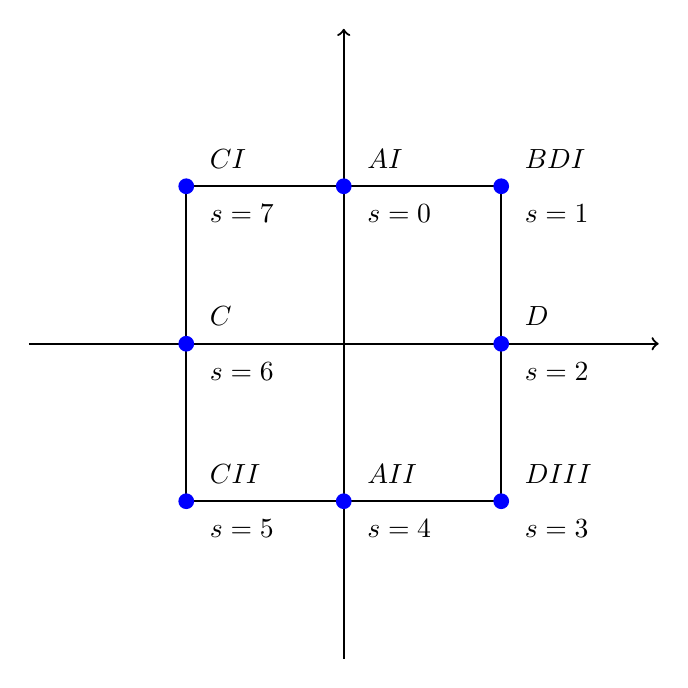
\begin{tikzpicture}
        \draw[->,thick](-4,0)--(-2,0)--(2,0)--(4,0);
        \draw[->,thick](0,-4)--(0,-2)--(0,2)--(0,4);
        \draw[thick](-2,-2)--(-2,2)--(2,2)--(2,-2)--cycle;
        \fill[blue] (0,2) circle (0.1);
        \node[above=1em,right=0.5em] at (0,2) {$AI$};
        \node[below=1em,right=0.5em] at (0,2) {$s=0$};
        \fill[blue] (2,2) circle (0.1);
        \node[above=1em,right=0.5em] at (2,2) {$BDI$};
        \node[below=1em,right=0.5em] at (2,2) {$s=1$};
        \fill[blue] (2,0) circle (0.1);
        \node[above=1em,right=0.5em] at (2,0) {$D$};
        \node[below=1em,right=0.5em] at (2,0) {$s=2$};
        \fill[blue] (2,-2) circle (0.1);
        \node[above=1em,right=0.5em] at (2,-2) {$DIII$};
        \node[below=1em,right=0.5em] at (2,-2) {$s=3$};
        \fill[blue] (0,-2) circle (0.1);
        \node[above=1em,right=0.5em] at (0,-2) {$AII$};
        \node[below=1em,right=0.5em] at (0,-2) {$s=4$};
        \fill[blue] (-2,-2) circle (0.1);
        \node[above=1em,right=0.5em] at (-2,-2) {$CII$};
        \node[below=1em,right=0.5em] at (-2,-2) {$s=5$};
        \fill[blue] (-2,0) circle (0.1);
        \node[above=1em,right=0.5em] at (-2,0) {$C$};
        \node[below=1em,right=0.5em] at (-2,0) {$s=6$};
        \fill[blue] (-2,2) circle (0.1);
        \node[above=1em,right=0.5em] at (-2,2) {$CI$};
        \node[below=1em,right=0.5em] at (-2,2) {$s=7$};
    \end{tikzpicture}
    \caption{周期性时钟}
\end{figure}
\begin{table}[h]
    \centering
    \begin{tabular}{|l|l|l|l|l|l|l|l|l|}
    \hline
    $s-\delta$ & 0   & 1           & 2           & 3 & 4    & 5 & 6 & 7 \\ \hline
    $K(s;d,D)$ & $Z$ & $Z_2^{(1)}$ & $Z_2^{(2)}$ & 0 & $2Z$ & 0 & 0 & 0 \\ \hline
    \end{tabular}
    \caption{周期表}
\end{table}

为了讨论具有拓扑非平凡态的一个可观察的结果,让我们回想一下,根据定义,如果严格执行对称条件,相图中的拓扑非平凡态和平凡态总是被量子相变分开的。这反过来意味着,如果拓扑绝缘体或拓扑超导体在空间上接近一个平凡相,那么在两相之间的边界上应该有一个无能隙的态。这种无能隙(即临界)状态可以被认为是由于空间中局部发生的相变而产生的,在这种相变中,哈密顿量的参数作为横向到边界方向的函数变化。这种无能隙边界模在这样的意义上得到了保护,即只要体隙不和对称性不被破坏,它们在扰动下是稳定的。特别是,无能隙边界模完全不受无序影响,完全规避Anderson局部化。这种无能隙边缘态的存在是拓扑绝缘体和拓扑超导体最显著的特征,实际上可以看作是拓扑绝缘体和拓扑超导体的定义。这种非平凡体拓扑性质和无能隙边模之间的紧密联系被称为体边对应

\subsubsection{拓扑缺陷}
将体拓扑绝缘体和拓扑超流体从物质的平凡态中分离出来的边界是余维1对象,即比体维数小一维,这些状态具有拓扑保护的无能隙模式。可以讨论一般更高余维的拓扑缺陷,如在能隙体系统中引入的点和线缺陷,以及它们的拓扑分类。绝热循环的拓扑性质也可以用类似的方式进行讨论。

拓扑缺陷最初是在自发对称破缺的背景下讨论的。例如,II型超导的量子通量涡旋涉及配对序参量的缠绕,打破了电荷守恒$U(1)$对称性。位错和滑移是与晶格介质中离散的扭转和曲率通量相关联的晶体缺陷,它打破了连续的平移和旋转对称性。它们都涉及缺陷周围某些序参量的非平凡长尺度调制。

拓扑带理论中的拓扑缺陷有不同的起源,因为它们不一定与自发对称破缺有关。例如,拓扑绝缘体和平凡绝缘体之间的质量间隙并不破坏任何对称。在能带理论中,它仍然是控制材料体拓扑的一个参数,我们将其称为能带参数或拓扑参数。因此,绝缘体和超导中的拓扑缺陷是缺陷周围这些拓扑参数的非平凡长尺度缠绕。

对于我们感兴趣的拓扑缺陷是由一个有缺陷的哈密顿描述的,它是一个在空间上由参量$r$缓慢调制的能带哈密顿$H_{r}(k)=H(k,r)$,其中包括空间坐标和/或时间参数。缺陷哈密顿量描述了缺陷周围的大尺度环境——距离缺陷很远。调制速度足够慢,使得与缺陷核心分离的体系统具有微观的时空平移对称性,因此可以用动量$k$来表征。更精确的讲,我们假设$\xi|\delta_rH(k,r)\leq \epsilon_h|$,其中$\xi$是类似于晶格间距或者类似于$1/\varepsilon_g$的时间微观特征长度,其中$\varepsilon_g$是能带体隙。TR、PH和CS对称性作用在缺陷哈密顿上为
\begin{equation}
    \begin{split}
        TH(k,r)T^{-1}=H(-k,r)\\
        CH(k,r)C^{-1}=-H(-k,r)\\
        SH(k,r)S^{-1}=-H(k,r)
    \end{split}
\end{equation}
其中空间参数$r$(当讨论绝热循环时是时间参数)是不变的,因为对称性作用在局域微观自由度上,它们与缓慢变化的调制无关。

不同的缺陷哈密顿可以用下列三个量来区分
\begin{enumerate}
    \item AZ对称类$s$
    \item 体维数$d$
    \item 缺陷的余维$d_c$,这是根据缺陷的维数$d_{defect}$定义的$d_c=d-d_{defect}$
\end{enumerate}
维数$d_{defect}$的空间缺陷被$D$维球面$S^{D}$包裹,其中$D=d_c-1=d-d_{defect}-1$. 例如三维空间中的一个点缺陷有余维$d_c=3-0=3$,因此被一个二维球面包络。绝热循环被合并为拓扑缺陷,依赖于循环时间参数。在这个情况下,缺陷被$S^{D-1}$球面包裹,在$d$维实空间里维数为$D-1=d-d_{defect}-1$. 算上在$S^1$上的时间参数,绝热循环被$D$维流形$S^{D-1}\times S^1$包围。

对于实AZ对称类,结果表明,拓扑缺陷的分类只依赖于一个数
\begin{equation}
    s-\delta=s-d-d_{defect}\quad mod\quad 8
\end{equation}
其中$\delta=d-D$被称为拓扑维,它在能隙拓扑绝缘体和拓扑超导的情况里扮演一个常用维数$d$的角色。对于空间缺陷,拓扑维依赖于缺陷维数$\delta=d-D=d_{defect}+1$并且与体维数$d$独立无关。例如点缺陷总有$\delta=1$,线缺陷总有$\delta=2$. 对于绝热循环,$D$分量参数$r$中的额外时间参数使拓扑维数减少1。例如,点缺陷的时间循环有$\delta=0$. 

两个复AZ类A和AIII中的拓扑缺陷以类似的方式分类,除了对称类现在存在于一个两个小时的周期时钟上,拓扑维数$\delta=d−D$以及数字$d−\delta$现在是模$2$的整数。当$\delta$是偶数(奇数),Class A(Class AIII)中的拓扑缺陷是整数类的。除此之外他们是平凡类。通过丢弃反幺正对称性,实AZ类分裂成两个复对称类
\begin{equation}
    \begin{split}
        &AI,D,AIII,C\rightarrow A\\
        &BDI,DIII,CI,CII\rightarrow AIII
    \end{split}
\end{equation}
其中手征算符$S$由TR和PH的乘积给出,这个过程依赖于实分类和复分类。例如,周期表中$s-\delta=4mod8$的$2Z$分类是根据相应的复$Z$分类归一化的。这意味着当丢弃反幺正对称时,$s−\delta=4$的拓扑不变量必须是偶数。

就像将体拓扑与边缘无能隙激发联系起来的体—边对应一样,我们也有一个体缺陷对应,它保证了体拓扑参数围绕缺陷的非平凡缠绕的无能隙缺陷激发。

\subsection{拓扑不变量}
在这一节中,我们根据体拓扑不变量讨论了能隙拓扑绝缘体和拓扑超导的十重分类和拓扑缺陷。将在下表中对讨论的拓扑不变量做简短总结。我们将讨论拓扑不变量和具有拓扑不变量特征的系统的各种具体例子,但我们主要局限于从能隙拓扑绝缘体和拓扑超导中选取的例子。拓扑缺陷的例子以后再讨论。

\begin{table}[h]
    \centering
    \begin{tabular}{|l|l|l|}
    \hline
                & Nonchiral classes(s even) & Chiral classes(s odd) \\ \hline
    $Z$         & 陈数                        & 缠绕数                   \\ \hline
    $Z_2^{(1)}$ & CS                        & Fu-Kane               \\ \hline
    $Z_2^{(2)}$ & Fu-Kane                   & CS                    \\ \hline
    \end{tabular}
    \caption{拓扑不变量分类表}
\end{table}

根据Bloch-BdG哈密顿量的本征函数给出了本节引入的拓扑不变量。我们把能级$\varepsilon^a$的本征函数记作$|u^a(k,r)\rangle$,$H(k,r)|u^a(k,r)\rangle=\varepsilon^a(k,r)|u^a(k,r)\rangle$. 通过假设,在$\varepsilon^a(k,r)$给出的能带结构中,在费米能量处存在一个能隙。我们假设在费米能量上下有$N_{+/-}$个带。总能带数为$N_++N_-$. 我们把满带Bloch函数记作$\{|u_-^\alpha(k,r)\rangle\}$或者简单记作$\{|u^\alpha(k,r)\}$,其中$\alpha=1,\cdots,N_-$.

布洛赫函数定义在$BZ^d\times\mathcal{M}^d$流形上,$(d+D)$维的总相空间由$(k,r)$参数化。这里$D$维流形$\mathcal{M}^D$围绕着这个拓扑缺陷。(它从缺陷的时空间的补形变收缩而来)例如,去掉实三维空间中的一个点缺陷,留下一个穿孔空间,该空间与$2$维球面$S^2$具有相同的同伦型。无现长线缺陷的补在三维空间中可以沿着缺陷方向压扁成一个有穿孔的盘子,然后变形回缩到圆$S^1$. 包围一个更加复杂的拓扑缺陷的$D$维流形$\mM^D$可能不会是一个球。例如,在三维空间中围绕连杆的是一个$T^2$。时间循环的流形$D$必须包含一个与周期时间方向相对应的不可收缩的1循环。本系列大部分中,我们感兴趣的是不涉及低维循环缺陷的最高维强拓扑。为此目的,通过收缩所有低维度的循环,我们将相空间紧化成一个球
\begin{equation*}
    (k,r)\in BZ^d\times\mM^D\xrightarrow{\text{紧化}}S^{d+D}
\end{equation*}
从物理上讲,这意味着缺陷能带理论假定在这些低维循环周围有平凡的缠绕。
\subsubsection{$s$为偶数的奇系:Chern数}
对于在非手征类($s$为偶数)能隙拓扑相和拓扑缺陷,整数$Z$分类的拓扑由Chern数表征
\begin{equation}
    Ch_n=\frac{1}{n!}\left(\frac{i}{2\pi}\right)^n\int_{BZ^d\times\mathcal{M}^D}Tr(\mathcal{F}^n)
\end{equation}
其中$n=(d+D)/2$. Berry曲率为
\begin{equation}
    \mathcal{F}=dA+A\wedge A
\end{equation}
这里用了微分形式:
\begin{equation}
    A^{\alpha\beta}=A_I^{\alpha\beta}(s)\mathrm{d}s^I,\quad A_I^{\alpha\beta}=\langle u^\alpha(s)|\partial_I u^\beta(s)\rangle
\end{equation}
\begin{equation}
    \begin{split}
        \mathcal{F}^{\alpha\beta}&=dA^{\alpha\beta}+A^{\alpha\gamma}\wedge A^{\gamma\beta}\\
        &=\partial_J A_I^{\alpha\beta}(s)\mathrm{d}s^J\wedge\mathrm{d}s^I+A_I^{\alpha\gamma}A_J^{\gamma\beta}\mathrm{d}s^I\wedge\mathrm{d}s^J\\
        &=\frac{1}{2}(\partial_IA_J^{\alpha\beta}(s)+[A_I^{\alpha\gamma},A_J^{\gamma\beta}])\mathrm{d}s^I\wedge \mathrm{d}s^J
    \end{split}
\end{equation}
其中$I,J=1,2,\cdots,d+D.$以及$s=(k,r)$. $A^{\alpha\beta}(k,r)$表示非阿贝尔联络
\begin{equation}
    \begin{split}
        A^{\alpha\beta}(k,r)&=\langle u^{\alpha}(k,r)|\mathrm{d}u^\beta(k,r)\rangle\\
        &=\langle u^\alpha(k,r)|\nabla_k u^\beta(k,r)\rangle\cdot \mathrm{d}k+\langle u^\alpha(k,r)|\nabla_r u^\beta(k,r)\rangle\cdot \mathrm{d}r
    \end{split}
\end{equation}
当$d+D$是偶数的时候,Chern数良定义。此外,在出现$TRS$或者$PHS$的系统里当$\delta=d-D=2\mod{4}$或者$0\mod{4}$时,Chern数为零。而且当$s-\delta=4\mod{8}$时,Chern数必定为偶数。

Chern数可以检测在底空间$BZ^d\times\mathcal{M}^D$上定义光滑Bloch波函数的障碍。与每一个$(k,r)$联系,我们有一个波函数$|u^a(k,r)\rangle$集合,一个可以被认为是$U(N_++N_-)$的一个元素的集合。然而,有一个规范冗余:对于给定的$(k,r)$在空带和占据带波函数中的$U(N_{\pm})$转动产生了相同的量子基态(费米狄拉克海)。换句话说,量子基态在给定的$(k,r)$中是陪集空间$U(N_++N_-)/U(N_-)\times U(N_+)$的一个元素,是复Grassmannian流形。费米狄拉克海可以很方便的用谱投影算符来表述
\begin{equation}
    P(k,r)=\sum_{\alpha=1}^{N_-}|u^\alpha(k,r)\rangle\langle u^\alpha(k,r)|
\end{equation}
或者写成指标显式$P^{ij}(k,r)=\sum_{\alpha=1}^{N_-}u_i^\alpha(k,r)[u_j^\alpha(k,r)]^*$,它指定了一个由占据带的布洛赫波函数的集合定义的总希尔伯特空间的子空间。投影算符是规范不变的并且是复Grassmannian流形的一个元素$P(k,r)\in U(N_++N_-)/(U(N_-)\times U(N_+))$. 对于下面的内容,引入$Q$矩阵是很方便的
\begin{equation}
    Q(k,r)=1-2P(k,r)
\end{equation}
$Q$矩阵是厄米的并且和$H(k,r)$有相同的本征函数集,但是他的本征值是$\pm 1$,因为$Q^2=1$.

当我们在底空间$BZ^d\times \mathcal{M}^D$移动的时候,波函数集合发生绝热变化。这样的波函数就定义了一个可以“扭曲”的纤维丛:在底空间各处都要找到定义良好的光滑波函数可能是不可能的。一个查看纤维丛什么时候扭曲的快速方法是注意到布洛赫函数的集合定义了一个从底空间到$U(N_++N_-)/(U(N_+)\times U(N_-))$的映射。这类拓扑上不同的映射可以用同伦群来分类
\begin{equation}
    \pi_{d+D}[U(N_++N_-)/(U(N_+)\times U(N_-))]
\end{equation}
对于足够大的$N_\pm$以及$d+D$是偶数的时候,$\pi_{d+D}[U(N_++N_-)/(U(N_+)\times U(N_-))]=Z$. 因此,拓扑上不同的映射具有整数拓扑不变量的特征,即
\begin{equation}
    -\frac{1}{2^{2n+1}}\frac{1}{n!}\left(\frac{i}{2\pi}\right)^n\int_{BZ^d\times \mathcal{M}^D}Tr[Q(\mathrm{d}Q)^{2n}]
\end{equation}
这不是什么,这正是Chern数。
\paragraph{例子:二维Class A量子反常霍尔效应}
作为一个例子,我们考虑$N_+=N_-=1$维数为$2$的带绝缘体。一般而言,二带布洛赫哈密顿可以根据四个实函数$R_{0,1,2,3}(k)$写成
\begin{equation}
    H(k)=R_0(k)\sigma_0+\mathbf{R}(k)\cdot \mathbf{\sigma}
\end{equation}
其中$\mathbf{R}=(R_1,R_2,R_3)$. 能带的能量色散关系为
\begin{equation}
    \varepsilon_{\pm}(k)=R_0(k)\pm R(k),\quad R(k)=|\mathbf{R}(k)|
\end{equation}
对于带绝缘体,在费米能处有一个能隙,为了方便起见,令此处的能量为$0$. 因此我们假设$R_0(k)+R(k)>0>R_0(k)-R(k)$,特别地,这意味着对于所有$k$都有$R(k)>0$

在这个二带的粒子里,布洛赫哈密顿$H(k)$或者四个矢量$R_{\mu=0,1,2,3}(k)$定义了从BZ到无约束四维向量$R_\mu$空间的映射。然而布洛赫波函数仅仅依赖单位矢量$\mathbf{n}(k)=\mathbf{R}(k)/R(k)$,这从以下两点很容易看到:
\begin{enumerate}
    \item $H(k)$中的$R_0(k)$并不会影响到波函数
    \item $\mathbf{R}(k)\cdot\mathbf{\sigma}=R(k)\mathbf{n}(k)\cdot\mathbf{\sigma}$
\end{enumerate}
从布洛赫波函数的这个观点出发,我们考虑一个从BZ到$S^2$上单位矢量$\mathbf{n}$的映射。后者是复Grassmannian流形的最简单的例子$U(2)/U(1)\times U(1)=S^2$

在二带模型中,不同的带绝缘体可以被不同的映射$\mathbf{n}(k)$表征。通过把BZ$T^2$紧化为$S^2$,拓扑上不同的映射可以利用二阶同伦群$\pi_2(S^2)$来分类,这给出了$\pi_2(S^2)=Z$. 对于给定的映射$\mathbf{n}$,整数拓扑不变量为
\begin{equation}\label{Chern num2}
    \frac{1}{4\pi}\int_{BZ}\mathbf{n}\cdot\mathrm{d}\mathbf{n}\times\mathrm{d}\mathbf{n}\in Z
\end{equation}
这可以计算出当我们扫过BZ时单位向量$\mathbf{n}$缠绕$S^2$的次数并且告诉我们$n$映射属于哪一个拓扑类。

现在让我们明确地构造布洛赫波函数。一个可能的选择是
\begin{equation}\label{wavefun1}
    |u^{\pm}\rangle=\frac{1}{\sqrt{2R(R\mp R_3)}}\begin{pmatrix}
        R_1-iR_2\\
        \pm R-R_3
    \end{pmatrix}
\end{equation}
观察占据带布洛赫函数$|u^-\rangle$在$\mathbf{R}=(0,0,-R)$处有一个奇点。当拓扑不变量\eqref{Chern num2}是非零的时候,矢量$\mathbf{n}(k)$必然将BZ中至少一个点映射到南极,因此,如果坚持在BZ中处处使用波函数\eqref{wavefun1},就会遇到奇点。从这个意义上说,在定义BZ中全局光滑良好的波函数时存在一个障碍。为了避免这个奇异性,我们可以把BZ分片,并且在不同片上用不同的波函数。例如在南极附近我们可以选择
\begin{equation}\label{wavefun2}
    |u^\pm\rangle=\frac{1}{\sqrt{2R(R\pm R_3)}}\begin{pmatrix}
        \pm R+R_3\\
        R_1+i R_2
    \end{pmatrix}
\end{equation}
这个波函数在南极是光滑的,但是在北极$\mathbf{R}=(0,0,R)$处是奇异的。利用两片波函数可以覆盖整个BZ。在两片交叠区域,两个波函数通过规范变换联系起来。

利用布洛赫波函数的显式形式,我们可以计算谱投影算符或者$Q$矩阵,并且可以看到不同的规范选择\eqref{wavefun1}和\eqref{wavefun2}产生相同的投影算符(投影算符规范不变),并且仅仅只依赖于$\mathbf{n}(k)$.

例如我们选择规范\eqref{wavefun1}
\begin{equation*}
    \begin{split}
        P&=|u^-\rangle\langle u^-|=\frac{1}{2R(R+R_3)}\begin{pmatrix}
            R_1-iR_2\\
            -R-R_3
        \end{pmatrix}\begin{pmatrix}
            R_1+iR_2&-R-R_3
        \end{pmatrix}\\
        &=\begin{pmatrix}
            \frac{R_1^2+R_2^2}{2R(R+R_3)}&-\frac{R_1-iR_2}{2R}\\
            -\frac{R_1+iR_2}{2R}&\frac{(R+R_3)^2}{2R(R+R_3)}
        \end{pmatrix}
    \end{split}
\end{equation*}
这样可以计算出$Q$矩阵
\begin{equation}
    Q=1-2P=\begin{pmatrix}
        \frac{R_3}{R}&\frac{R_1-iR_2}{R}\\
        \frac{R_1+iR_2}{R}&-\frac{R_3}{R}
    \end{pmatrix}=\frac{\mathbf{R}\cdot \bm{\sigma}}{R}
\end{equation}
Chern数为
\begin{equation*}
    \begin{split}
        Ch^1&=-\frac{i}{16\pi}\int_{BZ}Tr[Q\mathrm{d}Q\wedge \mathrm{d}Q]\\
        &=-\frac{i}{16\pi}\int_{BZ}Tr[Q(\frac{\partial Q}{\partial k_x}\frac{\partial Q}{\partial k_y}-\frac{\partial Q}{\partial k_y}\frac{\partial Q}{\partial k_x})]\mathrm{d}k_x\wedge \mathrm{d}k_y\\
        &=-\frac{i}{16\pi}\int_{BZ}Tr[\bm{\sigma}\cdot\mathbf{n}(\bm{\sigma}\cdot\frac{\partial\mathbf{n}}{\partial k_x}\bm{\sigma}\cdot\frac{\partial\mathbf{n}}{k_y}-\bm{\sigma}\cdot\frac{\partial\mathbf{n}}{\partial k_y}\bm{\sigma}\cdot\frac{\partial\bm{n}}{\partial k_x})]\mathrm{d}k_x\wedge\mathrm{d}k_y
    \end{split}
\end{equation*}
分为两项分别计算
\begin{equation}
    \begin{split}
        Term1&=\sigma_i n_i\sigma_j\frac{\partial n_j}{\partial k_x}\sigma_k\frac{\partial n_k}{\partial k_y}\\
        &=(\delta_{ij}+i\varepsilon_{ijk'}\sigma_{k'})\sigma_kn_i\frac{\partial n_j}{\partial k_x}\frac{\partial n_k}{\partial k_y}\\
        &=\sigma_k n_i\frac{\partial n_i}{\partial k_x}\frac{\partial n_k}{k_y}+i\varepsilon_{ijk}n_i\frac{\partial n_j}{\partial k_x}\frac{\partial n_k}{\partial k_y}-(\delta_{ki}\delta_{lj}-\delta_{kj}\delta_{li})\sigma_ln_i\frac{\partial n_j}{\partial k_x}\frac{\partial n_k}{\partial k_y}\\
        &=\mathbf{n}\cdot\frac{\partial\mathbf{n}}{\partial k_x}(\bm{\sigma}\cdot\frac{\partial\mathbf{n}}{\partial k_y})+i\varepsilon_{ijk}n_i\frac{\partial n_j}{\partial k_x}\frac{\partial n_k}{\partial k_y}-(\mathbf{n}\cdot\frac{\partial\mathbf{n}}{\partial k_y})(\bm{\sigma}\cdot\frac{\partial\mathbf{n}}{\partial k_x})+(\bm{\sigma}\cdot\mathbf{n})(\frac{\partial\mathbf{n}}{\partial k_x}\cdot\frac{\partial\mathbf{n}}{\partial k_y})\\
        Term2&=Term1(x\leftrightarrow y)
    \end{split}
\end{equation}
所以Chern数为(注意这里要Trace一个单位矩阵会多一个$2$倍)
\begin{equation}
    Ch^1=\frac{1}{8\pi}\int_{BZ}\mathbf{n}\cdot(\mathrm{d}\mathbf{n}\times\mathrm{d}\mathbf{n})
\end{equation}
利用Bloch波函数,我们可以计算Berry联络和Chern数,同样也可以得到上面的结果

这里展示一下计算过程,为了方便,我们依旧选取规范\eqref{wavefun1},因为规范的选取并不影响Berry Curvature的结果。这次我们在$\mathbf{R}$所在的$S^2$作为底流形上计算:
\begin{equation}
    \begin{split}
        Ch^1&=\frac{i}{2\pi}\int_{BZ}Tr(F)=\frac{i}{2\pi}\int_{BZ}Tr(\frac{1}{2}F_{\mu\nu}^{\alpha\beta}\mathrm{d}R^\mu\wedge\mathrm{d}R^{\nu})\\
        &=\frac{i}{4\pi}\int_{BZ}Tr(F_{\mu\nu}^{\alpha\beta})\mathrm{d}R^\mu\wedge\mathrm{d}R^\nu\\
        &=\frac{i}{4\pi}\sum_{\alpha}\int_{BZ}F_{\mu\nu}^{\alpha\alpha}\mathrm{d}R^\mu\wedge\mathrm{d}R^\nu\\
        &=\frac{i}{4\pi}\sum_{\alpha\beta}\int_{BZ}\frac{\langle u^\alpha|\partial_\mu H|u^\beta\rangle\langle u^\beta|\partial_\nu H|u^\alpha\rangle}{(E^\alpha-E^\beta)^2}\mathrm{d}R^\mu\wedge\mathrm{d}R^\nu\\
        &=\frac{i}{4\pi}\sum_{\alpha\beta}\int_{BZ}\frac{\langle u^\alpha|\sigma_\mu|u^\beta\rangle\langle u^\beta|\sigma_\nu|u^\alpha\rangle}{(E^\alpha-E^\beta)^2}\mathrm{d}R^\mu\wedge\mathrm{d}R^\nu
    \end{split}
\end{equation}
Chern数的Trace仅仅对占满的能带求和
\begin{equation}
    \begin{split}
        Ch^1&=\frac{i}{4\pi}\int_{S^2}\frac{\langle u^-|\sigma_i|u^+\rangle\langle u^+|\sigma_j|u^-\rangle}{(E^--E^+)^2}\mathrm{d}R^i\wedge\mathrm{d}R^j\\
        &=\frac{i}{4\pi}\int_{S^2}\frac{\langle u^-|i\varepsilon_{ijk}\sigma_k|u^-\rangle-\langle u^-|\sigma_i|u^-\rangle\langle u^-|\sigma^j|u^-\rangle}{4R^2}\mathrm{d}R^i\wedge\mathrm{d}R^j\\
        &=\frac{i}{4\pi}\int_{S^2}\frac{i\varepsilon_{ijk}R^k}{4R^3}\mathrm{d}R^i\wedge\mathrm{d}R^j\\
        &=\frac{i}{4\pi}\int_{S^2}\frac{i}{4}\varepsilon_{ijk}n^k\mathrm{d}n^i\wedge\mathrm{d}n^j\\
        &=\frac{i}{4\pi}\int_{BZ}\frac{i}{4}\varepsilon_{ijk}n^i(\frac{\partial n^i}{\partial k^\mu}\frac{\partial n^j}{\partial k^\nu}-\frac{\partial n^i}{\partial k^\nu}\frac{\partial n^j}{\partial k^\mu})\mathrm{d}k^\mu\wedge\mathrm{d}k^\nu\\
        &=\frac{i}{4\pi}\int_{BZ}\frac{i}{2}\varepsilon_{ijk}n^i(\partial_\mu n^i)(\partial_\nu n^j)\mathrm{d}k^\mu\wedge\mathrm{d}k^\nu
    \end{split}
\end{equation}
所以我们可以看到Berry Curvature为
\begin{equation}
    Tr(\mathcal{F}(\mathbf{k}))=\frac{i}{2}\varepsilon_{ijk}n^i(\partial_\mu n^i)(\partial_\nu n^j)\mathrm{d}k^\mu\wedge\mathrm{d}k^\nu
\end{equation}
这与之前用$Q$矩阵计算结果一样

二带模型非零Chern数的一个很显然的例子是
\begin{equation}
    \mathbf{R}(k)=\begin{pmatrix}
        -2\sin k_x\\
        -2\sin k_y\\
        \mu+2\sum_{i=x,y}\cos k_i
    \end{pmatrix}
\end{equation}
\begin{equation}
    H=\mathbf{R}\cdot \bm{\sigma}=\begin{pmatrix}
        \mu+2\sum_{i=x,y}\cos{k_i}&-2\sin k_x+2i\sin k_y\\
        -2\sin k_x-2i\sin k_y&-\mu-2\sum_{i=x,y}\cos k_i
    \end{pmatrix}
\end{equation}
分别有三个量子相变点,分别在$\mu=0,\pm 4$,对应有四个相,Chern数分别为
\begin{equation}
    Ch=\begin{cases}
        0\quad&(|\mu|>4)\\
        -1\quad&(-4<\mu<0)\\
        1\quad&(0<\mu<4)
    \end{cases}
\end{equation}
$d=2$维晶格上Chern数非零且无净磁场的带绝缘体通常称为Chern绝缘体,并表现出量子反常霍尔效应,这推广了在存在均匀磁场下的整数霍尔效应。Chern数不是什么别的,正是量子霍尔电导$\sigma_{xy}$.

\subsubsection{s为奇数的基础系:缠绕数}
对于Bloch-BdG哈密顿,只要$d+D$为偶数,Chern数总是可以被定义的(尽管它的允许值取决于对称类和δ)。另一方面,拓扑不变量只有在对称存在的情况下才能定义。一个例子是拓扑不变量缠绕数$\nu$,它仅仅在手征对称($\{H(k,r),U_S\}=0,U_S^2=1$)出现的情况下才能定义。简单起见,我们关注于$TrU_S=0$的情况,例如$N_+=N_-=N$.在不存在手性对称性的情况下,投影算符是复Grassmannian的一个元素,而在存在手性对称性的情况下,相关的空间是酉群$U(N)$. 这点可以从手征对称哈密顿的反对角形式看到
\begin{equation}
    H(k,r)=\begin{pmatrix}
        0&D(k,r)\\
        D^\dagger(k,r)&0
    \end{pmatrix}
\end{equation}
对应的,在这个基里,$Q$矩阵也是反对角的
\begin{equation}
    Q=1-2P(k,r)=\begin{pmatrix}
        0&q(k,r)\\
        q^\dagger(k,r)&0
    \end{pmatrix}
\end{equation}
这里稍微证明一下

选取$H$的一个基底$|u\rangle$满足$H|u\rangle=\varepsilon|u\rangle$,由于手征对称并且$TrU_S=0$,每一个能级$\varepsilon$的$|u\rangle$都有一个能量$-\varepsilon$的$U_S|u\rangle$对应。我们知道
\begin{equation}
    \begin{split}
        U_S|\alpha\rangle&=|\alpha\rangle\\
        U_S|\beta\rangle&=-|\beta\rangle
    \end{split}
\end{equation}
其中$|\alpha\rangle=|u\rangle+U_S|u\rangle,|\beta\rangle=|u\rangle-U_S|u\rangle$

这样我们可以到从$H$对角表象到CS表象下的变换关系
\begin{equation}
    \begin{split}
        |u\rangle=\frac{1}{2}(|\alpha\rangle+|\beta\rangle)\\
        |U_Su\rangle=\frac{1}{2}(|\alpha\rangle-|\beta\rangle)
    \end{split}
\end{equation}
计算$Q$矩阵得到
\begin{equation}
    Q=|U_Su\rangle\langle U_Su|-|u\rangle\langle u|=-\frac{1}{2}(|\alpha\rangle\langle\beta|-|\beta\rangle\langle\alpha|)=\begin{pmatrix}
        0&q(k,r)\\
        q^\dagger(k,r)&0
    \end{pmatrix}
\end{equation}
其中反对角块$q(k,r)$是一个幺正矩阵。因此$q$矩阵定义了一个从底流形$BZ^d\times \mathcal{M}^D$到李群流形$U(N)$的映射。拓扑上区分这类映射是用同伦群$\pi_{d+D}(U(N))$分类,这个同伦群在$d+D$为奇数时是非平凡的,例如$\pi_{d+D}[U(N)]=\mathbf{Z}$($N$足够大)。拓扑不同的映射是用缠绕数来表征的
\begin{equation}
    \begin{split}
        \nu_{2n+1}[q]&=\int_{BZ^d\times\mathcal{M}^D}\omega_{2n+1}[q]\\
        \omega_{2n+1}[q]&=\frac{(-1)^nn!}{(2n+1)!}\left(\frac{i}{2\pi}\right)^{n+1}Tr[(q^{-1}\mathrm{d}q)^{2n+1}]
    \end{split}
\end{equation}
其中$d+D=2n+1$是奇数。例如当$(d,D)=(1,0),(3,0)$我们有
\begin{equation}
    \begin{split}
        \nu_1&=\frac{i}{2\pi}\int_{BZ}\mathrm{d}kTr[q^{-1}\partial_k q]\\
        \nu_3&=\int_{BZ}\frac{\mathrm{d}^3k}{24\pi^2}\varepsilon^{\mu\nu\rho}Tr[(q^{-1}\partial_\mu q)(q^{-1}\partial_\nu q)(q^{-1}\partial_\rho q)]
    \end{split}
\end{equation}
这里$\partial_\mu=\partial_{k_\mu}$
\subsubsection{s为奇数的基础系:Chern-Simons}
我们现在引入另一个拓扑不变量,Chern-Simons不变量。这个不变量可以在$d+D=$奇数时定义,并且不像Chern数是量子化的。然而,在对称性存在的情况下,它可以取离散值。我们随后使用量化的CS不变量来描述第一代$Z_2$和第二代$Z_2$。这里我们看到$CS$不变量在出现手征对称性时也是量子化的。

Chern-Simons不变量由$d+D=2n+1$维里Chern-Simons形式$Q_{2n+1}$定义
\begin{equation}
    \mathcal{Q}_{2n+1}=\frac{1}{n!}\left(\frac{i}{2\pi}\right)^{n+1}\int_{0}^{1}Tr(\mathcal{AF}_{t}^n),\quad F_t=t\mathrm{d}\mathcal{A}+t^2\mathcal{A}^2=t\mathcal{F}+(t^2-t)\mathcal{A}^2
\end{equation}
对Chern-Simons形式在底流形上积分得到Chern-Simons不变量
\begin{equation}
    CS_{2n+1}[\mathcal{A}]=\int_{BZ^d\times\mathcal{M}^D}\mathcal{Q}_{2n+1}(\mathcal{A})
\end{equation}
例如对于$n=0,1,2$
\begin{equation}
    \begin{split}
        \mathcal{Q}_1(\mathcal{A})&=\frac{i}{2\pi}\int_0^1\mathrm{d}tTr(\mathcal{A})=\frac{i}{2\pi}Tr(\mathcal{A})\\
        \mathcal{Q}_3(\mathcal{A})&=\left(\frac{i}{2\pi}\right)^{2}\int_0^1\mathrm{d}tTr(\mathcal{A}(t\mathrm{d}\mathcal{A}+t^2\mathcal{A}^2))=-\frac{1}{4\pi^2}Tr(\frac{1}{2}\mathcal{A}\mathrm{d}\mathcal{A}+\frac{1}{3}\mathcal{A}^3)=-\frac{1}{8\pi^2}Tr(\mathcal{A}\mathrm{d}\mathcal{A}+\frac{2}{3}\mathcal{A}^3)\\
        \mathcal{Q}_5(\mathcal{A})&=\frac{1}{2}\left(\frac{i}{2\pi}\right)^3\int_0^1Tr(\mathcal{A}(t\mathrm{d}\mathcal{A}+t^2\mathcal{A}^2)^2)=-\frac{i}{16\pi^3}\int_0^1Tr(t^2\mathcal{A}(\mathrm{d}\mathcal{A})^2+2t^3\mathcal{A}^3\mathrm{d}\mathcal{A}+t^4\mathcal{A}^5)\\
        &=-\frac{i}{16\pi^3}Tr(\frac{1}{3}\mathcal{A}(\mathrm{d}A)^2+\frac{1}{2}\mathcal{A}^3\mathrm{d}\mathcal{A}+\frac{1}{5}\mathcal{A}^5)=-\frac{i}{48\pi^3}Tr(\mathcal{A}(\mathrm{d}\mathcal{A})^2+\frac{3}{2}\mathcal{A}^2\mathrm{d}\mathcal{A}+\frac{3}{5}\mathcal{A}^5)
    \end{split}
\end{equation}
Chern-Simons形式不是规范不变的。Chern-Simons的积分形式也不是。但是对于两个不同的规范选择$A$和$A^g$,它们由一个规范变换$g$连接
\begin{equation}
    A^g=g^{-1}Ag+g^{-1}\mathrm{d}g,\quad \mathcal{F}^g=g^{-1}\mathcal{F}g
\end{equation}
Chern-Simons形式的差$\mathcal{Q}_{2n+1}(A^g)-\mathcal{Q}_{2n+1}(A)$由缠绕数密度$\omega_{2n+1}[g]$和一个全导数项给出
\begin{equation}
    \mathcal{Q}_{2n+1}(A^g)-\mathcal{Q}_{2n+1}(A)=\omega_{2n+1}[g]+\mathrm{d}\alpha_{2n+1}(A,g)
\end{equation}
这样对于Chern-Simons形式的积分
\begin{equation}\label{CS integer}
    CS_{2n+1}[A^g]-CS_{2n+1}[A]=integer
\end{equation}
并且指数形式
\begin{equation}
    W_{2n+1}=\exp(2\pi i CS_{2n+1}[A])
\end{equation}
是良定义的,规范不变的量,虽然他不必要是量子化的。

到目前为止,讨论都是泛泛的。我们现在计算了手征对称存在下的CS不变。为此,我们首先明确地写下手征对称哈密顿量的Berry联络。对于给定的$q(k,r)$,本征函数可以显式的构造为
\begin{equation}
    |u^\alpha_\epsilon(k,r)\rangle_N=\frac{1}{\sqrt{2}}\begin{pmatrix}
        |n^\alpha\rangle\\
        \epsilon q^\dagger(k,r)|n^\alpha\rangle
    \end{pmatrix},\quad \epsilon=\pm
\end{equation}
在这个构造里,$Q$矩阵是对角的,对角元分别是$1,-1$. $|n^\alpha\rangle$是$N$个正交无关向量。为了简单,我们选择$(n^\alpha)_\beta=\delta_{\alpha\beta}$. 这些波函数没有任何奇异性,也就是说,我们明确地证明了整体的构造本征波函数没有障碍。Berry联络为
\begin{equation}
    \begin{split}
        A_N&=\langle u_\epsilon^\alpha|\mathrm{d}u_\epsilon^\alpha\rangle\\
        &=\frac{1}{2}\left[\langle n^\alpha|\mathrm{d}n^\alpha\rangle+\langle q^\dagger n^\alpha|\mathrm{d}q^\dagger n^\alpha\rangle+\langle q^\dagger n^\alpha|q^\dagger \mathrm{d}n^\alpha\rangle\right]\\
        &=\langle n^\alpha|\mathrm{d}n^\alpha\rangle+\frac{1}{2}\langle n^\alpha|q\mathrm{d}q^\dagger|n^\alpha\rangle=\frac{1}{2}q\mathrm{d}q^\dagger
    \end{split}
\end{equation}
在这个规范下,CS形式$\mathcal{Q}_{2n+1}$是缠绕数的一半,$\mathcal{Q}_{2n+1}(A_N)=\omega_{2n+1}[q^\dagger]/2$. 我们可以得到$CS_{2n+1}[A_N]=\nu_{2n+1}[q^\dagger]/2$
\begin{equation}
    W_{2n+1}=\exp(\pi i\nu_{2n+1}[q])=\pm 1
\end{equation}
也就是说,对于具有手征对称的哈密顿$W_{2n+1}$仅仅能取两个值$W_{2n+1}=\pm 1$

当$(d,D)=(1,0)$时,CS不变量$W_1$是定义在$BZ^d\simeq S^1$上的$U(1)$Wilson圈。$W_1$的对数表示电子极化,可以被手征对称性和反演对称性量子化。在这种情况下,$CS_1[A]$, \eqref{CS integer}的非不变性与这样一个事实有关:在周期系统中,电子坐标的位移只在一个单元内有意义,也就是说,两个坐标相差晶格常数的整数倍,应该是恒等的。

当$(d,D)=(3,0)$时,$CS_3$表示量子化的电磁极化率或者$\theta$角。$\theta$角,用Chern-Simons积分表示为
\begin{equation}
    \theta=2\pi\int_{BZ}\mathcal{Q}_3(k)\mod{2\pi}
\end{equation}
通过轴项$\delta S=(\frac{\theta\alpha}{4\pi})\int\mathrm{d}^3r\mathrm{d}t\mathbf{E}\cdot\mathbf{B}$出现在电动力学的有效作用中,其中$\alpha$是精细结构常数。量化的磁电极化率首先是在三维TR对称拓扑绝缘体$Class AII$的背景下被注意到的。除了TRS,手征对称和反演对称也能量子化CS不变量量$W_3$
\paragraph{例子:一维Class AIII聚合物}
考虑一个一维晶格上双粒子hopping模型
\begin{center}
    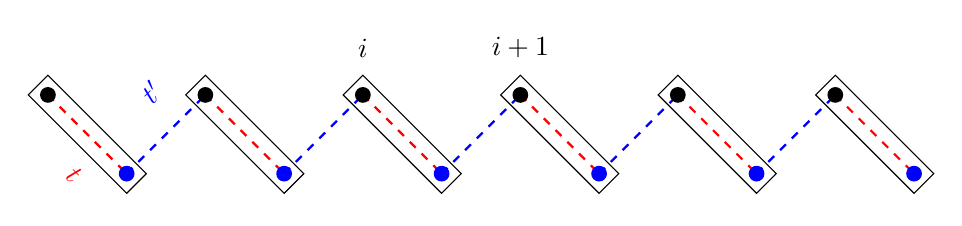
\begin{tikzpicture}
        \draw (-0.25,0) -- (1,-1.25) -- (1.25,-1) -- (0,0.25) -- cycle;
        \draw (1.75,0) -- (3,-1.25) -- (3.25,-1) -- (2,0.25) -- cycle;
        \draw (3.75,0) -- (5,-1.25) -- (5.25,-1) -- (4,0.25) -- cycle;
        \draw (5.75,0) -- (7,-1.25) -- (7.25,-1) -- (6,0.25) -- cycle;
        \draw (7.75,0) -- (9,-1.25) -- (9.25,-1) -- (8,0.25) -- cycle;
        \draw (9.75,0) -- (11,-1.25) -- (11.25,-1) -- (10,0.25) -- cycle;
        \draw[dashed,thick,red] (0,0) --node[below=1em,rotate=-45]{$t$} (1,-1);
        \draw[dashed,thick,red] (2,0) -- (3,-1);
        \draw[dashed,thick,red] (4,0) -- (5,-1);
        \draw[dashed,thick,red] (6,0) -- (7,-1);
        \draw[dashed,thick,red] (8,0) -- (9,-1);
        \draw[dashed,thick,red] (10,0) -- (11,-1);
        \draw[dashed,thick,blue] (1,-1) --node[above=1em,rotate=45]{$t'$} (2,0);
        \draw[dashed,thick,blue] (3,-1) -- (4,0);
        \draw[dashed,thick,blue] (5,-1) -- (6,0);
        \draw[dashed,thick,blue] (7,-1) -- (8,0);
        \draw[dashed,thick,blue] (9,-1) -- (10,0);
        \fill (0,0) circle (0.1);
        \fill (2,0) circle (0.1);
        \fill (4,0)node[above=1em]{$i$} circle (0.1);
        \fill (6,0)node[above=1em]{$i+1$} circle (0.1);
        \fill (8,0) circle (0.1);
        \fill (10,0) circle (0.1);
        \fill[blue] (1,-1) circle (0.1);
        \fill[blue] (3,-1) circle (0.1);
        \fill[blue] (5,-1) circle (0.1);
        \fill[blue] (7,-1) circle (0.1);
        \fill[blue] (9,-1) circle (0.1);
        \fill[blue] (11,-1) circle (0.1);
    \end{tikzpicture}
\end{center}
\begin{equation}
    \hat{H}=t\sum_{i}(a_i^\dagger b_i+h.c.)-t'\sum_{t}(b_i^\dagger a_{i+1}+h.c.)
\end{equation}
其中$a_i/b_i$是费米子在子格$A/B$上第$i$个原胞的湮灭算符。我们只考虑最近邻的hopping振幅为实数的情况,我们分别记作$t,t'$,其中我们假设$t,t'>0$. 这是描述乙炔的SSH模型。在动量空间中,哈密顿写成$\hat{H}=\sum_{k}\Psi^\dagger(k) H(k)\Psi(k)$, 其中$\Psi(k)=(a_k,b_k)^T,k\in[-\pi,\pi]$
\begin{equation}\label{lattice model}
    H(k)=\mathbf{R}(k)\cdot\bm{\sigma},\quad \mathbf{R}(k)=\begin{pmatrix}
        t-t'\cos k\\
        -t'\sin k\\
        0
    \end{pmatrix}
\end{equation}
能谱为$\varepsilon(k)=\pm\sqrt{t^2-2tt'\cos k+t'^2}$. 哈密顿有手征对称性,在动量空间里满足变换条件$\sigma_3 H\sigma_3=-H(k)$. 在这个对称性里,两个有能隙相$t>t'$和$t<t'$是拓扑可分辨的,并且被$t=t'$的量子相变点隔开。在$t>t'$相里的基态和原子绝缘体是绝热连通的。换句话说,一旦手征对称性引入,在$t'>t$相的基态与拓扑平凡原子绝缘体是拓扑区分的。这两个相由缠绕数来表征
\begin{equation}
    \nu[q]=\frac{i}{2\pi}\int_{BZ}\mathrm{d}k q^\dagger\partial_k q=\begin{cases}
        1,\quad t'>t\\
        0,\quad t'<t
    \end{cases}
\end{equation}
其中$q(k)=(t-t'e^{-ik})/|\varepsilon(k)|$. 简单计算一下
\begin{equation}
    \nu[q]=\frac{i}{2\pi}\int_{BZ}q^\dagger\mathrm{d}q=\frac{i}{2\pi}\int_{-\pi}^{\pi}\mathrm{d}k\partial_k\ln q=\left.\frac{i}{2\pi}\ln q\right|_{-\pi}^\pi
\end{equation}
\begin{equation}
    \ln q=\ln |q|+\arg q=\arg q,\quad |q|=1
\end{equation}
\begin{center}
    \begin{tikzpicture}
        \draw[->](-1,0)--(4,0);
        \draw[->](0,-2)--(0,2);
        \draw[blue] (2,0)circle(1);
        \draw (2,-0.1)node[below]{$t$}--(2,0.1);
        \draw[->](2,0)--(2.707,0.707)node[above]{$t'e^{-ik}$};
        \node[below=1em,left=0.5em] at (0,0) {$O$};
    \end{tikzpicture}
\end{center}
相应的CS不变量也有两个可区分的量子化值$1(0)$,分别对应$t'>t$和$t>t'$. 假设$t/t'$在相变点附近,SSH模型的低能物理是连续狄拉克哈密顿
\begin{equation}
    H(k)=-t'k\sigma_2+(t-t')\sigma_1
\end{equation}
这由$k$空间中的哈密顿在$k=0$处展开得到。注意到$t-t'$扮演着质量$m$的角色。

为了讨论domain wall,我们可以令$t\rightarrow t+m,t'\rightarrow t$. 更进一步说,我们让$m$是独立的,它定义了Class AIII和BDI哈密顿的一个缺陷
\begin{equation}
    H(k,r)=[t(1-\cos k)+m(r)]\sigma_1-t\sin k\sigma_2
\end{equation}
我们考虑一个受到空间调制的质量隙$m(r)$,它描述了一个domain wall的夹层,例如$m(r)=sgn(r)m_0,(|r|>R_0),m_0\neq 0$. 缠绕数为
\begin{equation}
    \begin{split}
        \nu_1&=\frac{i}{2\pi}\int_{BZ\times S^0}q^\dagger\mathrm{d}q\\
    \end{split}
\end{equation}
简单计算一下:
\begin{equation}
    H(k,r)=\mathbf{d}\cdot \sigma=\begin{pmatrix}
        &d_1-id_2\\
        d_1+id_2&
    \end{pmatrix}
\end{equation}
能量本征方程为
\begin{equation}
    \begin{pmatrix}
        &d_1-id_2\\
        d_1+id_2&
    \end{pmatrix}\begin{pmatrix}
        \alpha\\
        \beta
    \end{pmatrix}=\pm d\begin{pmatrix}
        \alpha\\
        \beta
    \end{pmatrix}
\end{equation}
\begin{equation}
    |u^\pm\rangle=\frac{1}{\sqrt{2}}\begin{pmatrix}
        \frac{d_1-id_2}{d}\\
        \pm 1
    \end{pmatrix}
\end{equation}
\begin{equation}
    Q=|u^+\rangle\langle u^+|-|u^-\rangle\langle u^-|=\begin{pmatrix}
        &\frac{d_1-id_2}{d}\\
        \frac{d_1+id_2}{d}&
    \end{pmatrix},\quad q=\frac{d_1-id_2}{d}
\end{equation}
\begin{equation}
    \begin{split}
        \nu_1&=\frac{i}{2\pi}\int_{BZ\times S^0}q^\dagger dq\\
        &=\frac{i}{2\pi}\int_{BZ}\mathrm{d}k[q^\dagger(k,R_0)\partial_k q(k,R_0)-q^\dagger(k,-R_0)\partial_k q(k,-R_0)]\\
        &=-\frac{1}{2\pi}[\arg q(k,R_0)|_0^{2\pi}-\arg q(k,-R_0)|_0^{2\pi}]
    \end{split}
\end{equation}
\begin{equation}
    d_1=t+m(r)-t\cos k,\quad d_2=-t\sin k,\quad d_1-id_2=t+m(r)-te^{-ik}
\end{equation}
\begin{center}
    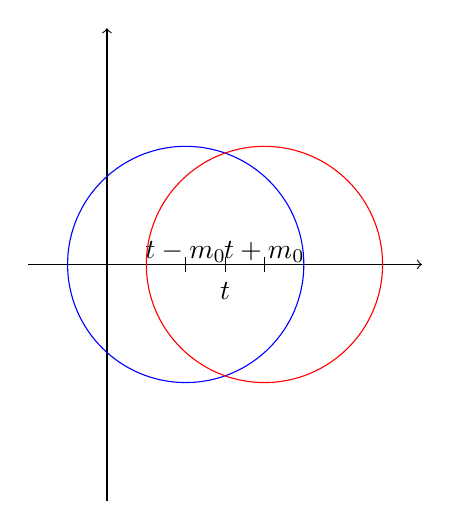
\begin{tikzpicture}
        \draw[->](-1,0)--(4,0);
        \draw[->](0,-3)--(0,3);
        \draw[blue](1,0)circle(1.5);
        \draw(1,-0.1)node[above]{$t-m_0$}--(1,0.1);
        \draw[red](2,0)circle(1.5);
        \draw(2,-0.1)node[above]{$t+m_0$}--(2,0.1);
        \draw(1.5,-0.1)node[below]{$t$}--(1.5,0.1);
    \end{tikzpicture}
\end{center}
其中$S^0=\{R_0,-R_0\}$是在原点处夹着缺陷点的两个点。该缺陷还以CS积分为特征,在这个例子里是电极化率
\begin{equation}
    CS_1=\frac{i}{2\pi}\int_{BZ\times S^0}\mathcal{A}=\frac{i}{2\pi}\int_{0}^{2\pi}\mathrm{d}k[A(k,R_0)-A(k,-R_0)]
\end{equation}
\begin{equation}
    A=\langle u^-|\partial_k|u^-\rangle=\frac{i}{2}\partial_k\ln q
\end{equation}
所以
\begin{equation}
    CS_1=-\frac{1}{2\pi}\frac{1}{2}[\arg q(k,R_0)|_0^{2\pi}-\arg q(k,-R_0)|_0^{2\pi}]=\frac{1}{2}\mod \mathbb{Z}
\end{equation}
上述两个不变量告诉我们domain wall两侧的不同。即使对于连续的Jackiw-Rebbi模拟,它们也有很好的定义
\begin{equation}
    H(k,r)=-tk\sigma_2+m(r)\sigma_1
\end{equation}
其中,在任何一边的体拓扑不变量在没有正规化的时候不会有整数值。然而上述两个不变量方程中所示的差异是正规无关的,并检测域壁处的局域零能量模式。  
\paragraph{3维Class DIII:$^3He-B$}
我们考虑BdG哈密顿为
\begin{equation}
    \hat{H}=\frac{1}{2}\sum_{k}\Psi^\dagger H(k)\Psi(k)
\end{equation}
其中$\Psi^\dagger=(\psi_{\uparrow}^\dagger,\psi_{\downarrow}^\dagger,\psi_{\uparrow},\psi_{\downarrow})$,
\begin{equation}
    \begin{split}
        H(k)&=\begin{pmatrix}
            \xi(k)&\Delta(k)\\
            \Delta(k)&-\xi(k)
        \end{pmatrix}\\
        \xi(k)&=k^2/2m-\mu,\quad \Delta(k)=\Delta_0i\sigma_2\mathbf{k}\cdot\bm{\sigma}
    \end{split}
\end{equation}
这个哈密顿具有PHS和TRS。属于ClassDIII,在三维情况下具有整数Chern数,由缠绕数表征。
\begin{equation}
    \nu[q]=\frac{1}{2}(sgn(\mu)+1)
\end{equation}
这是一个修正狄拉克型,直接套用沈顺清的结论$N=sgn(m)+sgn(B)$

具体计算参考沈老师文献和PHYSICAL REVIEW B 78, 195125 (2008). 下面我们复现一下PHYSICAL REVIEW B 78, 195125 (2008)中的计算。

对于三维狄拉克方程,我们讨论它可能有的拓扑分类
\begin{equation}
    H=-i\alpha^\mu \partial_\mu+m\beta
\end{equation}
其中$\alpha^\mu=\tau^1\otimes \sigma^\mu,\beta=\tau^3\otimes\sigma^0$
\begin{equation}
    \alpha^\mu=\tau^1\otimes\sigma^\mu=\begin{pmatrix}
        &\sigma^\mu\\
        \sigma^\mu&
    \end{pmatrix},\quad\beta=\tau^3\otimes\sigma^0=\begin{pmatrix}
        \sigma^0&\\
        &-\sigma^0
    \end{pmatrix}
\end{equation}
我们知道$\alpha^\mu=\gamma^0\gamma^\mu,\beta=\gamma^0$, 所以有
\begin{equation}
    \gamma^5=i\gamma^0\gamma^1\gamma^2\gamma^3=i\beta\beta\alpha^1\beta\alpha^2\beta\alpha^3=-i\alpha^1\alpha^2\alpha^3=\begin{pmatrix}
        &\sigma^0\\
        \sigma^0&
    \end{pmatrix}=\tau^1\otimes\sigma^0
\end{equation}
在动量空间中
\begin{equation}
    H(k)=\alpha^\mu k_\mu+m\beta=\begin{pmatrix}
        m&\mathbf{k}\cdot\bm{\sigma}\\
        \bm{k}\cdot\bm{\sigma}&-m
    \end{pmatrix}
\end{equation}
能谱色散关系为$E(k)=\pm\sqrt{k^2+m^2}=\pm \lambda(k)$. 这个四分量狄拉克方程一共有四种分类:Class AII、ClassAIII和ClassDIII

\textbf{ClassAII}: 四维狄拉克方程有一个时间反演不变性,其中时间反演算符的表示矩阵$U_T=-i\tau^0\otimes\sigma^2$
\begin{equation}
    U_T^{-1}H^*(k)U_T=H(k)
\end{equation}
验证一下
\begin{equation*}
    \begin{split}
        \begin{pmatrix}i\sigma^2&\\
        &i\sigma^2\end{pmatrix}\begin{pmatrix}
            m&(\bm{k}\cdot\bm{\sigma})^*\\
            (\bm{k}\cdot\bm{\sigma})^*&-m
        \end{pmatrix}\begin{pmatrix}
            -i\sigma^2&\\
            &-i\sigma^2
        \end{pmatrix}=\begin{pmatrix}
            m&\sigma^2(\bm{k}\cdot\bm{\sigma}^*)\sigma^2\\
            \sigma^2(\bm{k}\cdot\bm{\sigma}^*)\sigma^2&-m
        \end{pmatrix}
    \end{split}
\end{equation*}
利用$\sigma^2\bm{\sigma}^*=-\bm{\sigma}\sigma^2$. 可以得知
\begin{equation*}
    U_T^{-1}H^*(k)U_T=H(-k)
\end{equation*}
\textbf{ClassDIII}:除了TRS以外,狄拉克哈密顿还满足PHS,但是这里的PHS变换矩阵并不是ClassDIII里的标准形式,而是$\tau^2\otimes\sigma^2H^*(k)\tau^2\otimes\sigma^2=-H(-k)$. 为了解决这个问题,我们对哈密顿进行一个幺正变换
\begin{equation}
    H(k)\rightarrow\Omega H(k)\Omega^{-1}=\begin{pmatrix}
        m&(\bm{k}\cdot\bm{\sigma})i\sigma^2\\
        -i\sigma^2(\bm{k}\cdot\bm{\sigma})&-m
    \end{pmatrix},\quad \Omega=\begin{pmatrix}
        \sigma_0&\\
        &-i\sigma_y
    \end{pmatrix}
\end{equation}
简单推导一下这个幺正变换
\begin{equation*}
    \Omega H(k)\Omega^{-1}=\begin{pmatrix}
        \sigma^0&\\
        &-i\sigma^2
    \end{pmatrix}\begin{pmatrix}
        m&\bm{k}\cdot\bm{\sigma}\\
        \bm{k}\cdot\bm{\sigma}&-m
    \end{pmatrix}\begin{pmatrix}
        \sigma^0&\\
        &i\sigma^2
    \end{pmatrix}=\begin{pmatrix}
        m&(\bm{k}\cdot\bm{\sigma})i\sigma^2\\
        -i\sigma^2(\bm{k}\cdot\bm{\sigma})&-m
    \end{pmatrix}
\end{equation*}
\begin{equation*}
    \begin{split}
        &\tau^2\otimes\sigma^2H^*(k)\tau^2\otimes\sigma^2=-H(-k)\\
        &\Omega\tau^2\otimes\sigma^2\Omega^{-1}\Omega H^*(k)\Omega^{-1}\Omega\tau^2\otimes\sigma^2\Omega^{-1}=\Omega\tau^2\otimes\sigma^2\Omega^{-1}\begin{pmatrix}
            m&(\bm{k}\cdot\bm{\sigma})i\sigma^2\\
            -i\sigma^2(\bm{k}\cdot\bm{\sigma})&-m
        \end{pmatrix}\Omega\tau^2\otimes\sigma^2\Omega^{-1}
    \end{split}
\end{equation*}
计算一下
\begin{equation*}
    \Omega\tau^2\otimes\sigma^2\Omega^{-1}=\begin{pmatrix}
        \sigma^0&\\
        &-i\sigma^2
    \end{pmatrix}\begin{pmatrix}
        &-i\sigma^2\\
        i\sigma^2&
    \end{pmatrix}\begin{pmatrix}
        \sigma^0&\\
        &i\sigma^2
    \end{pmatrix}=\begin{pmatrix}
        0&\sigma^0\\
        \sigma^0&
    \end{pmatrix}=\tau^1\otimes\sigma^0
\end{equation*}
这就是标准的PHS变换形式,此时的哈密顿形式为
\begin{equation}
    \tilde{H}(k)=\begin{pmatrix}
        m&(\bm{k}\cdot\bm{\sigma})i\sigma^2\\
        -i\sigma^2(\bm{k}\cdot\bm{\sigma})&-m
    \end{pmatrix}
\end{equation}

PHS:$\tau^1\otimes\sigma^0H(k)\tau^1\otimes\sigma^0=-H^*(-k)$

TRS:$i\sigma^2H^*(k)(-i\sigma^2)=H(-k)$

例如氦3超流的BW相,BW相的$d$向量为$\bm{d}\propto\bm{k}$, $m$为化学势的负数$m=-\varepsilon_F=-\mu$

\textbf{ClassAIII}:三维狄拉克方程具有手征对称性,$\tau^2\otimes\sigma^0H(k)\tau^2\otimes\sigma^0=-H(k)$. 我们可以通过一个转动$\tau^2\rightarrow\tau^3$把手征算符块对角化
\begin{equation*}
    U^{-1}\tau^2U=\tau^3,\quad U=\frac{1}{\sqrt{2}}\begin{pmatrix}
        1&1\\
        i&-i
    \end{pmatrix}
\end{equation*}
在这个表象下,哈密顿是反对角形式:
\begin{equation*}
    H\rightarrow U^{-1}HU=\frac{1}{2}\begin{pmatrix}
        1&-i\\
        1&i
    \end{pmatrix}\begin{pmatrix}
        m&-i\sigma^\mu\partial_\mu\\
        -i\sigma^\mu\partial_\mu&-m
    \end{pmatrix}\begin{pmatrix}
        1&1\\
        i&-i
    \end{pmatrix}=-i\alpha^\mu\partial_\mu-i\beta\gamma^5m
\end{equation*}
在动量空间中
\begin{equation}
    H(k)=\begin{pmatrix}
        0&\bm{k}\cdot\bm{\sigma}-im\\
        \bm{k}\cdot\bm{\sigma}+im
    \end{pmatrix}
\end{equation}
手征对称性为$\beta H(k)\beta=-H(k)$. 对于能量$E(k)=-\lambda(k)$的情况,可以对$\bm{p}=0$的解进行一个Boost得到。具体计算可以参考我写的沈顺清笔记。

\begin{equation}
    \begin{split}
        |u_1(k)\rangle=\frac{1}{\sqrt{2\lambda(\lambda+m)}}\begin{pmatrix}
            -k_-\\
            k_z\\
            0\\
            \lambda+m
        \end{pmatrix},\quad |u_2(k)\rangle=\frac{1}{\sqrt{2\lambda(\lambda+m)}}\begin{pmatrix}
            -k_z\\
            -k_+\\
            \lambda+m\\
            0
        \end{pmatrix}
    \end{split}
\end{equation}
对于能量为正的情况$E(k)=\lambda(k)$
\begin{equation*}
    \begin{split}
        |u_3(k)\rangle=\frac{1}{\sqrt{2\lambda(\lambda-m)}}\begin{pmatrix}
            k_-\\
            -k_z\\
            0\\
            \lambda-m
        \end{pmatrix},\quad |u_4(k)\rangle=\frac{1}{\sqrt{2\lambda(\lambda-m)}}\begin{pmatrix}
            k_z\\
            k_+\\
            \lambda-m\\
            0
        \end{pmatrix}
    \end{split}
\end{equation*}
其中$k_\pm=k_x\pm ik_y$. 如果$m>0$,$|u_{3,4}(k)\rangle$在$\lambda(k)=m$处不是良定义的。($k=0$)

计算$Q$矩阵
\begin{equation}
    Q(k)=1-2P(k)=\frac{1}{\lambda}(k_\mu\alpha^\mu+m\beta)
\end{equation}
\begin{equation}
    Q(k)=|u_3\rangle\langle u_3|+|u_4\rangle\langle u_4|-|u_1\rangle\langle u_1|-|u2\rangle\langle u_2|=\frac{1}{\lambda}\begin{pmatrix}
        m&\bm{k}\cdot\bm{\sigma}\\
        \bm{k}\cdot\bm{\sigma}&-m
    \end{pmatrix}
\end{equation}
利用$\Omega$矩阵变到ClassDIII
\begin{equation}
    Q(k)\rightarrow\Omega Q(k)\Omega^{-1}=\frac{1}{\lambda}\begin{pmatrix}
        m&\bm{k}\cdot\bm{\sigma}(i\sigma^2)\\
        (-i\sigma^2)\bm{k}\cdot\bm{\sigma}&-m
    \end{pmatrix}
\end{equation}
然后利用$U$矩阵进入到手征表象中
\begin{equation}
    Q(k)=\frac{1}{\lambda}\begin{pmatrix}
        0&i\sigma^2(k_\mu\sigma^\mu-im)\\
        (k_\mu\sigma^\mu+im)(-i\sigma^2)&0
    \end{pmatrix}
\end{equation}
所以q矩阵为
\begin{equation}
    q(k)=i\sigma^2(k_\mu\sigma^\mu-im)
\end{equation}
利用缠绕数
\begin{equation}
    \nu[q]=\int_{BZ}\frac{\mathrm{d}^3k}{24\pi^2}\varepsilon_{\mu\nu\rho}Tr[(q^{-1}\partial_\mu q)(q^{-1}\partial_\nu q)(q^{-1}\partial_\rho q)]
\end{equation}
计算结果为
\begin{equation}
    \nu[q]=\frac{1}{2}sgn(m)
\end{equation}
\begin{mmaCell}[moredefined={s0, s1, s2, s3, s, k, inv, trace1, \
    trace2, ker, func},morefunctionlocal={k1, k2, k3},morepattern={k1_, \
    k2_, k3_}]{Input}
s0=\{\{1,0\},\{0,1\}\};
s1=\{\{0,1\},\{1,0\}\};
s2=\{\{0,-I\},\{I,0\}\};
s3=\{\{1,0\},\{0,-1\}\};
s=\{s1,s2,s3\};
k=\{\mmaUnd{k1},\mmaUnd{k2},\mmaUnd{k3}\};
inv=Inverse[k.s-I m s0];
trace1=Simplify[Tr[inv.s1.inv.s2.inv.s3]];
trace2=Simplify[Tr[inv.s3.inv.s2.inv.s1]];
ker=Simplify[\mmaFrac{(3trace1-3trace2)}{24\mmaSup{Pi}{2}}];
func[k1_,k2_,k3_]:=ker;
Integrate[func[k1,k2,k3],\{k1,-Infinity,Infinity\},\{k2,-Infinity,\
Infinity\},\{k3,-Infinity,Infinity\}]
\end{mmaCell}
\subsubsection{s为偶数的第一代$Z_2$}
对于奇序列,拓扑相或拓扑缺陷是由整Chern陈数来表征,对于第一或第二代拓扑相则是由$Z_2$拓扑不变量来表征。为了在一个统一的框架里讨论这些$Z_2$指标,我们采用两个策略:首先,我们从CS不变量出发,利用对称条件限制其可能值,构造各种$Z_2$拓扑不变量。其次,利用陈数和CS积分构造$Z_2$不变量。

第一代$Z_2$拓扑是由CS整数来表征
\begin{equation}\label{Z2CS}
    CS_{2n-1}=\int_{BZ\times\mathcal{M}^D}\mathcal{Q}_{2n-1}\in\frac{1}{2}\mathbb{Z}
\end{equation}
其中$2n-1=d+D$. CS不变量只定义了一个整数。注意在反幺正对称下,CS不变量通常可以取半整数值。当$CS_{2n−1}$为整数时,$Z_2$拓扑是平凡的;当$CS_{2n−1}$为半整数时,$Z_2$拓扑是非平凡的。

计算一般缺陷哈密顿量的CS积分时有一个微妙之处:它们需要一组在底流形上整体定义的占据态,这对于定义Chern数和缠绕数是不必要的。这种整体连续基可能存在拓扑障碍。特别是,当存在具有非零Chern不变量的非平凡弱拓扑时,整体的价标架不存在。在这种情况下,我们需要引入人造哈密顿$H(k,r)\rightarrow H(k,r)\oplus H_0(k,r_0)$去抵消弱拓扑同时不影响最高维强拓扑。这个可以被一个低维哈密顿$H_0(k,r_0)$来实现,其中$r_0$在一些恰当循环里$\mathcal{N}^{D'}\in\mathcal{M}^D$,不包围在考虑的缺陷。
\paragraph{一维Class D}
一维Class D的BdG哈密顿满足$C^{-1}H(-k)C=-H(k),C=\tau_1\mathcal{K}$,其中$k\in(-\pi,\pi]$是一维动量空间。ClassD的一维拓扑超导由CS积分表征。当有手征对称性时,PHS量子化$W=\exp(2\pi iCS[A])$为$\pm 1$。为了看到这点,我们回想起如果$|u_-^\alpha(k)\rangle$是负能解,能量为$-\varepsilon(k)$,那么$|\tau_1u^{*\alpha}_-(-k)\rangle$是正能解,能量为$\varepsilon(k)$. 负能和正能的Berry联络的关系为
\begin{equation}
    A_-^{\alpha\beta}(k)=\langle u_-^\alpha(k)|\partial_k u_-^\beta(k)\rangle=\langle u_-^\alpha(k)|C^{-1}C\partial_k C^{-1}C|u_-^\beta(k)\rangle=\langle \tau_1u_-^{\alpha*}(k)|\partial_k|\tau_1u_-^{\beta*}(k)\rangle=A_+^{\alpha\beta}(-k)
\end{equation}
一维CS积分为
\begin{equation}
    \begin{split}
        \int_{-\pi}^{\pi}\mathrm{d}kTrA_-&=\int_{0}^\pi\mathrm{d}kTrA_-(k)+\int_{-\pi}^0\mathrm{d}kTrA_-(k)\\
        &=\int_0^\pi\mathrm{d}kTrA_-(k)+\int_{0}^\pi\mathrm{d}kTrA_-(-k)\\
        &=\int_0^\pi\mathrm{d}kTr[A_-(k)+A_+(k)]\\
        &=\int_0^\pi\mathrm{d}ku_i^{a*}\partial_k u_i^{a}=\int_0^\pi\mathrm{d}kTr[U^\dagger\partial_kU]\\
        &=\int_0^\pi\mathrm{d}kTr\partial_k\ln U=\int_0^\pi\mathrm{d}k\partial_k\ln\det U=\ln\det U(\pi)-\ln\det U(0)
    \end{split}
\end{equation}
其中当$\alpha$跑遍所有能带的一半时(例如负能能带),$a$跑遍所有的能带。这里我们引入一个幺正矩阵符号$U_i^a(k)=u_i^a(k)$. 所以我们有CS不变量
\begin{equation}
    \begin{split}
        \mathcal{Q}_1(A)&=\frac{i}{2\pi}\int_0^1\mathrm{d}tTr(\mathcal{A})=\frac{i}{2\pi}\mathcal{A}\\
        CS_1[A]&=\int_{BZ}\mathcal{Q}_1(\mathcal{A})=\frac{i}{2\pi}\int_{-\pi}^{\pi}\mathrm{d}kA_-(k)=\frac{i}{2\pi}\ln\frac{\det U(\pi)}{\det U(0)}\\
        W&=e^{2\pi iCS_1[A]}=\frac{\det U(0)}{\det U(\pi)}
    \end{split}
\end{equation}
在PH对称动量$k=0,\pi$处,幺正矩阵$U(k)$有特殊性质。这个利用马约拉纳基很容看到。通过马约拉纳基变换,我们得到马约拉纳表象的哈密顿$X(k)$。回想起在TRIM点有PHS关系$\tau_1H^*(k)\tau_1=-H(-k)=-H(k)$. 因此,$X(k=0,\pi)$是一个实斜对称阵,可以通过一个正交变换$O(k=0,\pi)$变换到正则形式。注意在其他动量点没有$\tau_1H^T(k)\tau_1=H(k)$,马约拉纳哈密顿就不是斜对称阵。
\begin{equation}
    iX(k=0,\pi)=\Omega H(k=0,\pi)\Omega^\dagger,\quad\Omega=\begin{pmatrix}
        1&1\\
        i&-i
    \end{pmatrix},\quad X^T(k=0,\pi)=-X(k=0,\pi)
\end{equation}
\begin{equation}
    X(k=0,\pi)=O^T(k=0,\pi)\Sigma O(k=0,\pi),\quad\Sigma=\begin{pmatrix}
        0&\varepsilon_1\\
        -\varepsilon_1&0\\
        &&\ldots\\
        &&&0&\varepsilon_N\\
        &&&-\varepsilon_N&0
    \end{pmatrix}
\end{equation}
我们知道$U_i^a=\{|u_i^a\rangle\}$,并且
\begin{equation}
    HU_i^a=\varepsilon_i^a U_i^a\Rightarrow\Omega H\Omega^{-1}\Omega U_i^a=\varepsilon_i^a\Omega U_i^a\Rightarrow iX\Omega U_i^a=\varepsilon_i^a\Omega U_i^a\Rightarrow iO^T\Sigma O\Omega U_i^a=\varepsilon_i^a\Omega U_i^a\Rightarrow i\Sigma O\Omega U_i^a=\varepsilon_i^aO\Omega U_i^a
\end{equation}
$\Sigma$的本征向量是不含$k$的,所以$O\Omega$把哈密顿基底组$\{|u_i^a(k)\rangle\}$变成一组不含$k$的基底组,所以
\begin{equation}
    W=\frac{\det O(0)}{\det O(\pi)}
\end{equation}
由于$O(k=0,\pi)$是正交矩阵,他们的行列式是$\pm 1$,所以CS不变量$W=\pm 1$. 由于$2n$维斜方阵的Pfaffian为
\begin{equation}
    Pf(X)=\frac{1}{2^n n!}\sum_{\sigma\in S_n}(-1)^{|\sigma|}X_{\sigma(1)\sigma(2)}\cdots X_{\sigma(2n-1),\sigma(2n)}
\end{equation}
$\sigma$是$1,\cdots,2n$的全排列,我们注意到
\begin{equation}
    Pf(OXO^T)=Pf(X)\det(O),\quad\mathrm{sgn}(Pf(X(k))\det(O(k)))=\mathrm{sgn}(Pf(OXO^T))=1
\end{equation}
\begin{equation}
    W=\frac{\det O(0)}{\det O(\pi)}=\frac{Pf(\Sigma(0))}{Pf(X(0))}\frac{Pf(X(\pi))}{Pf(\Sigma(\pi))}=\mathrm{sgn}(Pf[X(0)]Pf[X(\pi)])
\end{equation}
很显然,这是规范不变的,与选择的底流形上的基函数无关。
\paragraph{Class D的Kitaev链}
Kitaev提出的一维拓扑超导激发了许多关于Majorana物理的研究。在一些最近的实验中观察到一维链中存在马约拉纳模的证据。Kitaev链的哈密顿为
\begin{equation}
    H=\frac{t}{2}\sum_{i}(c_i^\dagger c_{i+1}+c_{i+1}^\dagger c_i)-\mu\sum_{i}(c_i^\dagger c_i-\frac{1}{2})+\frac{1}{2}\sum_{i}(\Delta^*c_i^\dagger c_{i+1}^\dagger-\Delta c_ic_{i+1})
\end{equation}
不失一般性,$\Delta$可以取实数,因为整体序参量有一个$U(1)$规范,$\Delta=e^{i\theta}\Delta_0$. 在动量空间
\begin{equation}
    \hat{H}=\frac{1}{2}\sum_{k}\begin{pmatrix}
        c_k^\dagger&c_{-k}
    \end{pmatrix}H(k)\begin{pmatrix}
        c_k\\
        c_{-k}^\dagger
    \end{pmatrix},\quad H(k)=(t\cos k-\mu)\tau_3-\Delta_0\sin k\tau_2
\end{equation}
对于$|t|>\mu$和$|t|<\mu$有被相变点$t=\pm\mu$隔开的能隙相。Kitaev链可以根据Majorana基写成
\begin{equation}
    \lambda_j=c_j^\dagger+c_j,\quad \lambda_j'=i(c_j-c_j^\dagger),\quad\Lambda=\begin{pmatrix}
        \lambda_j\\
        \lambda_j'
    \end{pmatrix}=\Omega\Psi,\quad \Omega=\begin{pmatrix}
        1&1\\
        i&-i
    \end{pmatrix}
\end{equation}
上式进行傅里叶变换得到
\begin{equation}
    \lambda_k=c_{-k}^\dagger+c_k,\quad\lambda'_k=i(c_k-c_{-k}^\dagger)
\end{equation}
\begin{equation}
    \Lambda(k)=\begin{pmatrix}
        \lambda_k\\
        \lambda_k'
    \end{pmatrix},\quad\Lambda^\dagger(k)=\begin{pmatrix}
        \lambda_k^\dagger&\lambda_{k}'^\dagger
    \end{pmatrix}=\begin{pmatrix}
        \lambda_{-k}&\lambda_{-k}'
    \end{pmatrix}=\lambda^T(-k)
\end{equation}
所以在马约拉纳表象下哈密顿为
\begin{equation}
    \hat{H}=\frac{i}{2}\sum_{k}\Lambda^\dagger(k)X(k)\Lambda(-k)
\end{equation}
\begin{equation}
    iX(k)=\Omega^{-1}H(k)\Omega=(t\cos k-\mu)\tau_2-\Delta_0\sin k\tau_1
\end{equation}
所以CS不变量为
\begin{equation}
    W=\mathrm{sgn}(Pf[X(0)]Pf[X(\pi)])=\mathrm{sgn}(\mu^2-t^2)
\end{equation}
与SSH模型相似,我们也通过改变$\mu$作为空间的函数来考虑domian wall,它捕获了局域零能马约拉纳模。
\paragraph{三维Class AII}
我们现在讨论三维时间反演不变的拓扑性质。这些带式绝缘体的拓扑特性与TRS下哈密顿量的不变性密切相关$T^{-1}H(k)T=H(-k)$。由于这个关系,布洛赫波函数在$k$点与$-k$点是联系的。如果$|u^\alpha(k)\rangle$是$k$处的本征态,则$T|u^\alpha(k)\rangle$是$-k$的本征态。假设我们现在可以在BZ全空间上定义光滑的$|u^a(k)\rangle$.(这是可能的,因为时间反演不变性导致Chern数为$0$,没有拓扑障碍)我们比较$|u^\alpha(-k)\rangle$和$T|u^\alpha(k)\rangle$。 因为$|u^\alpha(-k)\rangle$和$T|u^a(k)\rangle$是同一个哈密顿$H(-k)$的本征态,他们之间一定由一个幺正矩阵联系起来
\begin{equation}
    |u^\alpha(-k)\rangle=[w^{\alpha\beta}(k)]^*|Tu^\beta(k)\rangle
\end{equation} 
$w$上的复共轭符合共同的约定。因此斜矩阵
\begin{equation}
    w^{\alpha\beta}(k)=\langle u^\alpha(-k)|Tu^\beta(k)\rangle
\end{equation}
由动量为$-k$的占据态与动量为$k$的占据的时间反演之间的交叠给出,在定义$Z_2$指数时起着重要作用。矩阵元服从
\begin{equation}
    w^{\alpha\beta}(-k)=\langle u^a(k)|T u^\beta(-k)\rangle=\langle T^2 u^\beta(-k)|Tu^a(k)\rangle=-w^{\beta\alpha}(k)
\end{equation}
所以在$k$和$-k$之间Berry联络有关系
\begin{equation}
    \begin{split}
        A_\mu^{\alpha\beta}(-k)&=\langle u^\alpha(-k)|\partial_\mu|u^\beta(-k)\rangle\\
        &=\langle T u^{\alpha'}(k)|w^{\alpha'\alpha}(k)\partial_\mu\left([w^{\beta\beta'}(k)]^*|Tu^{\beta'}(k)\rangle\right)\\
        &=\langle u^{\beta'}(k)|[w^{\alpha'\alpha}(k)]^*\partial_\mu w^{\beta\beta'}(k)|u^{\alpha'}(k)\rangle\\
        &=[w^{\alpha'\alpha}(k)]^*\partial_\mu w^{\beta\beta'}(k)\delta^{\beta'\alpha'}+\langle u^{\beta'}(k)|[w^{\alpha'\alpha}(k)]^*w^{\beta\beta'}(k)\partial_\mu|u^{\alpha'}(k)\rangle\\
        &=-w(k)\partial_\mu w^\dagger(k)-w(k)A_\mu^*(k)w^\dagger(k)
    \end{split}
\end{equation}
也就是$-A_\mu(-k)$和$A^*_\mu(k)=-A^T_\mu(k)$通过规范变换相互联系。

有了对Berry联络的这个约束,我们现在证明CS不变量是由斜矩阵的缠绕数$\omega[w]$给出的

上式的规范变换我们可以写成
\begin{equation}
    -A_\mu(-k)=[A_\mu^{g^*}]^*,\quad g=w^\dagger
\end{equation}
我们把CS积分变量做一个替换$k\rightarrow -k$
\begin{equation}
    CS[A(k)]=CS[A(-k)]=-CS[(A^{g^*})^*]=-(CS[A^{g^*}])^*=-CS[A^{g^*}]
\end{equation}
我们知道在规范变换$g$下,CS积分核有关系
\begin{equation}
    \mathcal{Q}_{2n+1}(A^g)-\mathcal{Q}_{2n+1}(A)=\omega_{2n+1}[g]+\mathrm{d}\alpha_{2n+1}(A,g)
\end{equation}
所以在上述规范变换下
\begin{equation}
    CS[A^{g^*}]-CS[A]=\int_{BZ}\{\omega[g^*]+\mathrm{d}\alpha(A,g^*)\}\Rightarrow CS[A]=-\frac{1}{2}\int_{BZ}\{\omega[g^*]+\mathrm{d}\alpha(A,g^*)\}
\end{equation}
所以$CS[A]=\frac{\mathbb{Z}}{2}$. 在BZ的TRIM点$K$处,规范矩阵$w$的Pfaffian也可以将CS不变量写成
\begin{equation}
    W=\prod_{K}\frac{Pf[w(K)]}{\sqrt{\det[w(K)]}}
\end{equation}
\subsubsection{s为偶的第二代$Z_2$}
Fu-Kane不变量适用于非手征对称类的第二代$Z_2$,由
\begin{equation}\label{sedFK}
    FK_n=\frac{1}{n!}\left(\frac{i}{2\pi}\right)^n\int_{BZ_{1/2}^d\times\mathcal{M}^D}Tr(\mathcal{F}^n)-\oint_{\partial BZ^d\times\mathcal{M}^D}\mathcal{Q}_{2n-1}
\end{equation}
定义,其中$n=(d+D)/2$. 它涉及到半布里渊区$BZ^d_{1/2}$上的Berry曲率的开积分,其中一个动量参数,比如$k_1$,跑遍$[0,\pi]$使得$BZ_{1/2}^d$的补空间是它的时间反演共轭。$BZ_{1/2}^d$上的CS积分,即$k_1=0,\pi$处的一半BZ的边界是规范相关的,在选择基时需要特别注意。对于时间反演系统(Class AI、Class AII),构造Berry联络$\mathcal{A}^{\alpha\beta}$的占据态$|u^\alpha(k,r)\rangle$需要满足规范条件
\begin{equation}\label{gauge condition}
    w^{\alpha\beta}(k,r)=\langle u^\alpha(-k,r)|Tu^\beta(k,r)\rangle=const
\end{equation}
对于$(k,r)\in\partial BZ_{1/2}^d\times \mathcal{M}^D$. 例如,描述2维Class AII拓扑绝缘体的原始FK不变量要求$w(k,r)=i\sigma_2$。对于PHS系统(Class D和C),占据态$|u^\alpha(k,r)\rangle$通过PH算符$C$生成非占据态$|v^\alpha(k,r)\rangle$. FK不变量的CS形式需要从占据态满足下列条件构造
\begin{equation}\label{occupied state}
    \int_{\partial BZ_{1/2}^d\times\mathcal{M}^D}Tr[(XdX^\dagger)^{d+D-1}]=0
\end{equation}
其中$X(k,r)=(u^1,\cdots,u^N,v^1,\cdots,v^N)$是由本征态构造的幺正矩阵。规范约束条件\eqref{gauge condition}和\eqref{occupied state}对于方程\eqref{sedFK}中的FK不变量是必须的。没有它们,CS积分可以通过占据态一个大的规范变换$|u^\alpha\rangle\rightarrow g_{\alpha\beta}|u^\beta\rangle$改变任意整数。规范条件约束了这样的变换使得CS项仅仅只能改变偶数。FK不变量因此取$\mathbb{Z}_2=\{0,1\}$
\paragraph{2维Class AII}
二维时间反演对称拓扑绝缘体的拓扑不变量是FK不变量。正如在三维时间反演对称拓扑绝缘体的情况一样,$\mathbb{Z}_2$不变量表达式可以为
\begin{equation}
    W=\prod_{k}\frac{\mathrm{Pf}[w(K)]}{\sqrt{\det w(K)}}
\end{equation}
其中$K$跑遍所有二维时间反演不变点。这个拓扑不变量可以被写成不同形式。例如可以被时间反演不变极化来引入,这可以在动量空间中被写成$SU(2)$Wilson loop.
\subsubsection{s为奇数的第一代$\mathbb{Z}_2$}
手征类的第一代$Z_2$与非手征类的第二代$Z_2$具有同构关系。这个关系在后面会详细讨论。对于手征类拓扑不变量$Z_2^{(1)}$因此是由规范约束条件\eqref{gauge condition}(s=1,5 CI,DIII)和\eqref{occupied state}(s=3,7 BDI,CII)给出
\paragraph{二维Class DIII}
正如二维时间反演对称拓扑绝缘体(Class AII)的情况,对于时间反演对称拓扑超导FK不变量可以由Pfaffian公式写出
\begin{equation}
    w(K)=\frac{\mathrm{Pf}(w(K))}{\sqrt{\det w(K)}}
\end{equation}
TRS的出现允许我们定义$Z_2$不变量。Pfaffian公式可以由$Q$矩阵给出。为了看到这个,我们在反对角块基底下写出BdG哈密顿
\begin{equation}
    H(k)=\begin{pmatrix}
        0&D(k)\\
        D^\dagger(k)&0
    \end{pmatrix},\quad D(k)=-D^T(-k)
\end{equation}
在这个表象中,TR算符由$T=U_T\mathcal{K}=i\sigma_2\otimes\mathbb{1}\mathcal{K}$给出,$Q$矩阵写成
\begin{equation}
    Q(k)=\begin{pmatrix}
        0&q(k)\\
        q^\dagger(k)&0
    \end{pmatrix},\quad q(k)=-q^T(-k)
\end{equation}
为了计算$Z_2$拓扑数,我们选择基底$|u_\pm^\alpha(k)\rangle_N$, 斜矩阵由$w^{\alpha\beta}(k)=-q^{\alpha\beta}(-k)$给出。$Z_2$拓扑数可以被表示成
\begin{equation}
    W=\prod_{K}\frac{\mathrm{Pf}[q(K)]}{\sqrt{\det[q(K)]}}
\end{equation}
在这里我想证明一下上述式子。对于一般的Class DIII而言
\begin{equation}
    H(k)=\begin{pmatrix}
        \xi(k)&\Delta(k)\\
        \Delta^\dagger(k)&-\xi^T(-k)
    \end{pmatrix}
\end{equation}
其中$\Delta(k)=-\Delta^T(-k)$. 对于Class DIII超导而言,TRS算符$U_T$和PHS算符$U_C$分别满足$U_T^2=-1,U_C^2=1$. 其中时间反演关系
\begin{equation}
    U_T^\dagger H^*(k)U_T=H(-k)
\end{equation}
其中$U_T=diag(u_T,u_T^*)$,在这里的基底$u_T=i\sigma_y$. 由于时间反演关系
\begin{equation}
    \begin{pmatrix}
        u_T^\dagger\\
        &u_T^T
    \end{pmatrix}\begin{pmatrix}
        \xi^*(k)&\Delta^*(k)\\
        \Delta^T(k)&-\xi^\dagger(-k)
    \end{pmatrix}\begin{pmatrix}
        u_T&\\
        &u_T^*
    \end{pmatrix}=\begin{pmatrix}
        u_T^\dagger\xi^*(k)u_T&u_T^\dagger\Delta^*(k)u_T^*\\
        u_T^T\Delta^T(k)u_T&-u_T^T\xi^\dagger(-k)u_T^*
    \end{pmatrix}
\end{equation}
所以有
\begin{equation}
    \begin{cases}
        u_T^\dagger\xi(k)u_T=\xi(-k)\\
        u_T^\dagger\Delta^*(k)u_T^*=\Delta(-k)
    \end{cases}
\end{equation}
利用$u_Tu_T^T=\mathbb{1}$和$u_T^T=-u_T,u_T^\dagger=-u_T$可以得到$u_T\Delta^\dagger(k)=\Delta(k)u_T^\dagger$. 手征算符为$U_S=U_TU_C=\tau_x\otimes i\sigma_2$

利用幺正变换$V$可以计算出手征表象下的哈密顿形式
\begin{equation}
    H(k)\rightarrow V^\dagger H(k)V=\begin{pmatrix}
        0&D(k)\\
        D^\dagger(k)&0
    \end{pmatrix}
\end{equation}
其中$V$为
\begin{equation}
    V=\frac{1}{\sqrt{2}}\begin{pmatrix}
        1&1\\
        iu_T&-iu_T
    \end{pmatrix}
\end{equation}
最后计算结果为$D(k)=h(k)+i\Delta(k)u_T^\dagger$. 时间反演对称要求
\begin{equation}
    u_T D^T(-k)u_T^\dagger=D(k),D^T(-k)=-D(k)
\end{equation}
此时Q矩阵为
\begin{equation}
    Q(k)=\begin{pmatrix}
        0&q(k)\\
        q^\dagger(k)&0
    \end{pmatrix},\quad q(k)=-q^T(-k)
\end{equation}
规范矩阵
\begin{equation}
    w^{\alpha\beta}(k)=\langle u^\alpha_+(-k)|\mathcal{T}u^\beta_+(k)\rangle
\end{equation}
其中$u_a^\pm(k)$是$Q$矩阵第$\alpha$个本征值为$\pm$本征态。根据手征哈密顿可以构造本征态
\begin{equation}
    |u^\alpha_\pm(k)\rangle_N=\frac{1}{\sqrt{2}}\begin{pmatrix}
        |n^\alpha\rangle\\
        \pm q^\dagger(k)|n^\alpha\rangle
    \end{pmatrix}
\end{equation}
或者可以选择为
\begin{equation}
    |u^\alpha_\pm(k)\rangle_S=\frac{1}{\sqrt{2}}\begin{pmatrix}
        \pm q(k)|n^\alpha\rangle\\
        |n^\alpha\rangle
    \end{pmatrix}
\end{equation}
其中$n^\alpha$是独立正交向量,为了简单起见,我们选择$(n^\alpha)_\beta=\delta_{\alpha\beta}$.
\begin{equation}
    \begin{split}
        w^{\alpha\beta}(k)&=\frac{1}{2}\begin{pmatrix}
            \langle n^\alpha|&\langle n^\alpha| q(-k)
        \end{pmatrix}T\begin{pmatrix}
            |n^\beta\rangle\\
            q^\dagger(k)|n^\beta\rangle
        \end{pmatrix}\\
        &=\frac{1}{2}\begin{pmatrix}
            \langle n^\alpha|&\langle n^\alpha| q(-k)
        \end{pmatrix}i\sigma_2\mathcal{K}\begin{pmatrix}
            |n^\beta\rangle\\
            q^\dagger(k)|n^\beta\rangle
        \end{pmatrix}\\
        &=\frac{1}{2}\begin{pmatrix}
            \langle n^\alpha|&\langle n^\alpha|q(-k)|
        \end{pmatrix}\begin{pmatrix}
            q^T(k)|n^\beta\rangle\\
            -|n^\beta\rangle
        \end{pmatrix}\\
        &=\frac{1}{2}(\langle n^\alpha|q^T(k)|n^\beta\rangle-\langle n^\alpha|q(-k)|n^\beta\rangle)\\
        &=\frac{1}{2}(\langle n^\alpha|q^T(k)|n^\beta\rangle+\langle n^\alpha|q^T(k)|n^\beta\rangle)\\
        &=q^T_{\alpha\beta}(k)
    \end{split}
\end{equation}
所以$Z_2$不变量为
\begin{equation}
    W=\prod_{K}\frac{\mathrm{Pf}[q^T(K)]}{\sqrt{\det [q(K)]}}
\end{equation}
\subsubsection{对于s为奇数的第二代$Z_2$}
对于手征类的第二代$Z_2$是由CS积分$CS_{2n-1}$所给出,其中$n=(d+D+1)/2$. 类似于FK不变量,CS形式在这里需要由占据态来构建,对于CI和DIII要满足规范条件\eqref{Z2CS},对于BDI和CII要满足规范条件\eqref{occupied state}. 连同反幺正对称,这个规范约束迫使Chern-Simions不变量\eqref{CS integer}是一个整数。如果$CS_{2n-1}$是偶数,$Z_2$是拓扑平凡的,如果$CS_{2n-1}$是奇数,$Z_2$是拓扑非平凡的。
\paragraph{一维Class DIII}
在$d=1$里,规范约束条件自动满足。CS积分成为极化率,并且有整数值。在手征表象基里,CS积分可以化简为$Z_2$不变量:
\begin{equation}
    (-1)^\nu=\frac{\mathrm{Pf}[q(\pi)]}{\mathrm{Pf}[q(0)]}\frac{\sqrt{\det[q(0)]}}{\sqrt{\det[q(\pi)]}}
\end{equation}
这依赖于在固定动量点$k=0,k=\pi$的信息。注意到$\sqrt{\det[q(k)]}$必须在这两个固定动量点之间是连续的。一维CS积分和上述方程等价的证明在Teo and Kane (2010b).证明里。作为一个粒子,我们考虑下列形式的Class DIII
\begin{equation}
    D(k)=-t\sin k\sigma_1-i[\Delta+u(1-\cos k)]\sigma_2
\end{equation}
其中$k\in[-\pi,\pi]$并且有$u\ll |\Delta|$
\begin{equation}
    (-1)^\nu=\frac{\mathrm{Pf}[q(\pi)]}{\mathrm{Pf}[q(0)]}\frac{\sqrt{\det[q(0)]}}{\sqrt{\det[q(\pi)]}}=\mathrm{sgn}(\Delta)
\end{equation}
\subsection{K理论}
在本节中,我们推导了能隙拓扑相和拓扑缺陷的分类,总结在表I中。拓扑分类可以由分类空间的同伦群或者K理论展示。我们也展示了Clifford代数在证明对称允许狄拉克质量项的分类空间中的应用。该方法利用了K理论与Clifford代数之间的已知联系,有效地将拓扑问题转化为代数问题;利用Clifford代数证明了K理论的Bott周期性。K理论的Bott周期律由Clifford代数证明。对于K理论、克利福德代数和博特周期性的更完整和精确的描述,可以参考数学和物理方面的文献。
\subsubsection{狄拉克质量隙的同伦分类}
我们已经看到,许多拓扑上的非平凡相(以及平凡相)都有一个有质量的狄拉克哈密顿量表示。人们可能更关注于狄拉克表示的分类。有人可能会认为这是一个粗略的近似,但事实证明,通过这种方式缩小自己所关注的不会失去太多。因此,我们考虑了Bloch-BdG哈密顿在相关动量点$K_0$附近的低能量描述,它一般采用Dirac形式  
\begin{equation}
    H(k,r)=k\cdot\Gamma+m\Gamma_0(r)
\end{equation}
其中$k=(k1,\cdots,k_d)$是距离动量点$K_0$的差值并且$\Gamma=(\Gamma_1,\cdots,\Gamma_d)$是狄拉克矩阵,满足Clifford关系$\{\Gamma_\mu,\Gamma_\nu\}=2\delta_{\mu\nu},(\mu,\nu=0,\cdots,d)$. 质量项$m\Gamma_0$依赖于一个$D$维空间参数$r$,它与所有动能项上的狄拉克矩阵是反对易的,并造成了一个体隙。对于一个稳定的分类,它是独立且对无关平凡带的添加不敏感,狄拉克矩阵的维数(带的数目)是足够大的,$\ln[dim(\Gamma_0)]\ll d+D$,其动机稍后将变得清晰。在存在对称的情况下,狄拉克矩阵满足
\begin{equation}\label{k,t}
    T\Gamma_0(r)T^{-1}=\Gamma_0(r),\quad T\Gamma T^{-1}=-\Gamma
\end{equation}
\begin{equation}
    C\Gamma_0(r)C^{-1}=-\Gamma_0(r),\quad C\Gamma C^{-1}=\Gamma
\end{equation}
\begin{equation}
    S\Gamma_0(r)S^{-1}=-\Gamma_0(r),\quad S\Gamma S^{-1}=-\Gamma
\end{equation}
对于一般的TI或TSC,质量项$mΓ_0$存在于某个参数空间$\mathcal{R}$中,该空间与某个分类空间具有相同的拓扑(或伦型),证明很简短。假设我们在两个体区域$A,B$之间有一个domain wall. 例如,二维系统里分离Chern绝缘体和普通绝缘体的domain wall可以在拓扑上捕获,其中质量项在界面上改变其符号。现在在$A,B$上分别选取两个任意点$r_A,r_B$. 如果在$\mathcal{R}$中不存在任何连接$m\Gamma(r_A)$和$m\Gamma(r_B)$的连续的路径,Domain wall 承载一个拓扑保护的表面模式。这个拓扑因此由$\pi_0(\mathcal{R})=[S^0,\mathcal{R}]$来表征,$\mathcal{R}$的$0$阶同伦群计算了连通片数。

对于除domain wall之外的一般拓扑缺陷,我们首先用狄拉克哈密顿量来近似缺陷哈密顿量,其中$r$现在是在时空中围绕缺陷的调制参数。在这种情况下,我们感兴趣的是最高维的强拓扑,其中$r$存在于(或变形收缩到)紧化球体$S^D$上。

对于不同的对称类$s$和体维数$d$,质量项$m\Gamma_0$属于不同的类空间$\mathcal{R}_{s-d}$. 正如我们将要看到的,类空间是由对称性\eqref{k,t}决定的。现在让我们用几个例子来演示这一点。
\paragraph{d=2,d=1中的Class A}
作为第一个例子,我们确定了Class A中与2D Chern绝缘体相关的分类空间。为此,我们首先回顾一下由\eqref{lattice model}给出的格点模型。在$K_0=0$附近线性化,我们得到$d=2$有质量狄拉克模型$H(k)=k_x\sigma_1+k_y\sigma_2+m\sigma_3$. 对于$m>0$和$m<0$有两个可分辨相,它的Chern数相差$1$. 为了讨论更一般的Chern数值,我们把哈密顿矩阵维数增大到$2N\times 2N$为狄拉克哈密顿
\begin{equation}
    H(k,r)=k_x\sigma_x\otimes\mathbf{1}_N+k_y\sigma_2\otimes\mathbf{1}_N+M
\end{equation}
因为质量项与动能项反对易,$M$应该有$\sigma_3\otimes A$的形式,其中$A$是$N\times N$的厄密矩阵。通过考虑$A=diag(m1,\cdots,m_N)$, $m_i\neq 0$,我们可以实现相对Chern数不同值的带绝缘体。这些只是$N$个不同质量的狄拉克绝缘体的解耦复制。质量的大小并不影响Chern数,然而质量的符号$\mathrm{sgn}m_i$与Chern数有关。所以不失一般性,我们考虑$A=\Lambda_{n,N-n}$, 其中$\Lambda_{n,m}=diag(\mathbf{1}_n,-\mathbf{1}_m)$. 从$\Lambda_{n,N-n}$出发,更一般的质量矩阵可以由幺正矩阵$U$做变换$A=U\Lambda_{n,N-n}U^\dagger$生成。相反的,对于给定$A$,只要他的本征值是恰当归一的,我们总可以通过幺正矩阵$U$来对角化并且写出$A=U\Lambda_{n,N-n}U^\dagger$. 因此,$A$是$U(N)/[U(n)\times U(N-n)]$的群元素。两个有相同正则形式的质量$A_1$和$A_2$是相互幺正联系的,例如,$U(N)/[U(n)\times U(N-n)]$是简单连通的。然而两个有不同正则形式的$A_1$和$A_2$没有幺正联系。总结来说,对于给定$N$,质量的集合是$U(N)/[U(n)\times U(N-n)]$

到目前为止,我们已经固定$N$,但这对于实现狄拉克表示所有可能的相是显然不够的,因为对于给定$N$,Chern数最大可以为$N$,而$d=2$ Class A的绝缘体可以被任意整Chern数来表征。为了实现任意Chern数的绝缘体,我们把$N$取得尽可能大,这让我们认为
\begin{equation}
    \mathcal{C}_0=\bigcup_{n=0}^{N}\frac{U(N)}{U(n)\times U(N-n)}\stackrel{N\rightarrow\infty}{\longrightarrow} BU\times \mathbb{Z}
\end{equation}
该空间的不连通分量$\pi_0(\mathcal{C}_0)$是拓扑质量不同的空间,已知为$\pi_0(\mathcal{C}_0)=\mathbb{Z}$。这与Class A在$d=2$的分类一致。

这里介绍一下Bott周期定理:
\begin{theorem}[Bott周期定理]
    令$U=U(\infty)$无穷维$U$群。则$U$的同伦群$\pi_i(U)$关于$i$是$2$周期的
\begin{equation}
    \begin{cases}
        \pi_{2k-1}(U)\simeq\pi_{2k+1}(U)=\mathbb{Z}\\
        \pi_{2k}\simeq \pi_{2k+2}(U)=0
    \end{cases}\quad \forall k=1,2,\cdots
\end{equation}
\end{theorem}

上面这个定理是由Bott同构定理支撑的
\begin{theorem}[Bott同构定理]
    复Grassmannian $G_m(\mathbb{C}^{2m})$与$SU(2m)$之间具有如下关系:
    \begin{enumerate}
        \item $SU(2m)$上连接单位矩阵$I$与$-I$的所有最小测地线构成空间
        
        $BSU(2m)=\{\gamma:[0,1]\rightarrow SU(2m)|\gamma\text{是连接$I$与$-I$的最小测地线}\}$与$G_m(\mathbb{C}^{2m})$同构,$BSU(2m)\simeq G_m(\mathbb{C}^{2m})$
        \item $SU(2m)$上连接$I$与$-I$的道路空间$\Omega SU(2m,I,-I)$中每一个非最小测地线$\gamma$的指标$Ind(\gamma)\geq 2m+2$
        \item $BSU(2m)$到$\Omega SU(2m)$的包含映射诱导出同构
        \begin{equation}
            \pi_i(G_m(\mathbb{C}^{2m}))\simeq \pi_i(\Omega SU(2m,I,-I)),\quad \forall i\leq 2m
        \end{equation}
        利用道路纤维化同伦序列可以得到
        \begin{equation}
            \pi_i(G_m(\mathbb{C}^{2mn}))\simeq \pi_{i+1}(SU(2m)),\quad \forall i\leq 2m
        \end{equation}
    \end{enumerate}
\end{theorem}

事实上,我们取无限个能带的极限,可以通过添加任意多的轨道来实现,这是K理论的一个重要组成部分。一般来说,平凡原子带的加入不会影响间隙相的非平凡拓扑性质。因此,人们一般对不包含平凡带的拓扑性质是稳定的感兴趣。然而,只有当带的数目限制为某个特定的整数时,间隙相的拓扑区别才会存在。例如,我们知道在具有任意带数的三维空间中不存在非平凡Class A拓扑绝缘体。然而,如果我们把自己限制在二带模型中,非平凡拓扑的存在是由非平凡同伦群\footnote{$\mathbb{C}P^1$对于$U(2)$是齐性流形,$U(1)$是迷向子群,所以有$\mathbb{C}P^1\simeq U(2)/U(1)$}$\pi_3(\mathbb{C}P^1)=\mathbb{Z}$所支持的,它对平凡带的添加是不稳定的。通过取无穷多个带的极限,我们消除了以下这种不稳定或偶然的拓扑,即,我们感兴趣的是有间隙的非相互作用系统基态的稳定等价性。

对可能的质量进行分类的问题可以用另一种方法表述如下。首先,狄拉克动力学项(没有质量的部分)由伽玛矩阵组成,形成Clifford代数。一般来说,一个复Clifford代数$Cl_n$是由一组生成元$\{e_i\}_{i=1,\cdots,n}$,它们满足:
\begin{equation}
    \{e_i,e_j\}=2\delta_{ij}
\end{equation}
复的意思是指它们可以用复矩阵来表示。(更正式的来说,我们感兴趣的是一个$2^n$维复向量空间$\{C_{p_1p_2\cdots}e_1^{P_1}e_2^{p_2}\cdots\}$,其中$p_i=0,1$,$C_{p_1p_2\cdots}$是复数。)对于存在二维$Class A$的例子,动能项狄拉克矩阵满足$\{\sigma_i,\sigma_j\}=2\delta_{ij}(i,j=1,2)$,它们构成$Cl_2$. 质量应该与动能项里所有的狄拉克矩阵反对易$\{\sigma_i,M\}=0$,算上质量,我们现在有$Cl_3$. 当考虑质量,我们通过添加一个生成元(质量)把代数从$Cl_2$扩张到$Cl_3$. 计算代数扩张的不同方法只不过是计算不等价幺正质量。

在一般情况下,我们首先考虑一组对称算子(和狄拉克动能项)。它们被表示为Clifford代数的生成元。然后我们考虑,除了这些生成元,还可能的质量项,这反过来扩张了Clifford代数。也就是说,对于对称生成元的固定表示,我们需要寻找新的附加生成元($=$质量)的可能表示矩阵。这些表示的集合形成了一个分类空间。拓扑上不同的状态对应于不同的代数扩张。  

再举一个例子,我们考虑一维Class A以及他们对于给定$H(k)=k_x\sigma_3\otimes\mathbf{1}_{N}+M$. 如之前,质量必须与狄拉克动能项反对易$\{\sigma_3,M\}=0$. 一般的解为
\begin{equation}
    M=\begin{pmatrix}
        0&U^\dagger\\
        U&0
    \end{pmatrix},\quad U\in U(N)
\end{equation}
对于固定的$N$,$\pi_0(U(N))=0$,所有的质量都可以相互的连续形变。也就是说没有拓扑可分辨的相。和前面一样,这个问题可以表述为一个扩张问题$Cl_1\rightarrow Cl_2$. 扩张分类空间为
\begin{equation}
    \mathcal{C}_1=U(N)
\end{equation}
同伦群为$\pi_0(\mathcal{C}_1)=0$.

这个解析可以在任意维数$d$重复。考虑扩张$Cl_d\rightarrow Cl_{d+1}$. 我们寻找$\pi_0(\mathcal{C}_d)$,表示对应的分类空间$\mathcal{C}_d$。由于$Cl_{n+2}\simeq Cl_n\otimes \mathbb{C}(2)$, 其中$\mathbb{C}(2)$是$2\times 2$复矩阵的代数空间,我们有分类空间的性质
\begin{equation}
    \mathcal{C}_{n+2}\simeq\mathcal{C}_n
\end{equation}
由此得出Class A拓扑分类的二重周期性。
\paragraph{Class AIII}
可以看出,给定对称类的拓扑分类问题的维数周期性直接来源于Clifford代数。类似地,由于增加了一个对称而引起的分类中的维数变化,也可以用Clifford代数来理解。举个例子,让我们考虑对称Class AIII中的零维系统,它的质量(即哈密顿量本身)$H$满足手性对称关系$\{H,U_S\}=0$. 幺正矩阵$U_S$,就像狄拉克动动能项中的$\Gamma$矩阵,可以被认为是Clifford生成元。通过适当的归一化(谱扁平化),零维哈密顿量H具有特征值$\pm 1$,可以认为是一个附加的Clifford生成元。我们考虑一个扩张问题$Cl_1\rightarrow Cl_2$,它的分类空间是$\mathcal{C}_1$并且$\pi_0(\mathcal{C}_1)=0$. 这样,对称性的存在可以被看成添加了一个合适数量的Clifford生成元,并且从效果上来看与添加空间维度一样。
\paragraph{d=0,1,2的Class D}
到目前为止,我们讨论了用复Clifford代数来分类Class A和Class AIII的狄拉克质量。实Clifford代数与狄拉克质量在八个实对称类中的分类有关,正如我们现在所说明的。

例如我们从$0$维的$Class D$出发,考虑哈密顿$H(r)=m\Gamma_0(r)$, 它与$C=\mathcal{K}$反对易。
\begin{equation}
    \{H(r),C\}=0\Rightarrow m(\Gamma_0(r)+\Gamma_0^*(r))\mathcal{K}=0\Rightarrow \Gamma_0(r)=-\Gamma_0^*(r)
\end{equation}
令$u_1,\cdots,u_N$是$\Gamma_0$正本征向量。由于$PHS$,$u_1^*,\cdots,u_N^*$是对应的负本征向量。
\begin{equation}
    \Gamma_0(r)\rightarrow u_1,\cdots,u_N
\end{equation}
\begin{equation}
    \Gamma_0(r)u_j=u_j\Rightarrow C\Gamma_0(r) u_j=Cu_j\Rightarrow C\Gamma_0(r)C^{-1}Cu_j=Cu_j\Rightarrow \Gamma_0^*(r)u_j^*=u^*_j
\end{equation}
\begin{equation}
    \Gamma_0(r)u_j^*=-u_j^*
\end{equation}
令$a_j,b_j$分别是$u_j$的实部和虚部,$u_j=\frac{1}{\sqrt{2}}(a_j+ib_j)$. 正交关系为
\begin{equation}
    \begin{cases}
        u_i^\dagger u_j=\delta_{ij}\\
        u_i^T u_j=0
    \end{cases}
\end{equation}
可以得到$a_i^T a_j=b_i^Tb_j=\delta_{ij},a_i^Tb_j=0$. 这样我们有一个$O(2N)$矩阵$A=(a_1,\cdots,a_N,b_1,\cdots,b_N)$. 注意到由于$U(N)$基变换$u_j\rightarrow u_j'=U_{jk}u_k$,相同的$\Gamma_0$可以对应于不同的正交矩阵$A$. 因此$d=0$中的$Class D$质量项$\Gamma_0$存在于分类空间
\begin{equation}
    \mathcal{R}_2=O(2N)/U(N)
\end{equation}

在一维情况,我们考虑
\begin{equation}
    H(k,r)=k\Gamma_1+m\Gamma_0(r)
\end{equation}
通过选择合适的基底,我们可以假设$PH$算符有$C=\mathcal{K}$形式,以及$\Gamma_1=\tau_3\otimes \mathbf{1}_N$. 根据\eqref{k,t}可以得到对称算符与$\Gamma$矩阵之间的关系为
\begin{equation}
    \{C,\Gamma_0(r)\}=0,\quad \{\Gamma_1,\Gamma_0(r)\}=0,\quad [C,\Gamma_1]=0
\end{equation}
所以我们有
\begin{equation}
    \{\Gamma_1,\Gamma_0\}\Rightarrow \Gamma_0=\tau_2\otimes\gamma_1+\tau_1\otimes i\gamma_2
\end{equation}
\begin{equation}
    \{C,\Gamma_0\}=0\Rightarrow \Gamma_0+\Gamma_0^*=0\Rightarrow \gamma_1=\gamma_1^*,\gamma_2=\gamma_2^*
\end{equation}
所以$\gamma_1$和$\gamma_2$是实矩阵。再根据$\Gamma_0=\Gamma_0^\dagger$我们得到
\begin{equation}
    \Gamma_0^\dagger=\tau_2\otimes\gamma_1^T-\tau_1\otimes i\gamma_2^T=\tau_2\otimes\gamma_1+\tau_1\otimes i\gamma_2
\end{equation}
我们有
\begin{equation}
    \gamma_1=\gamma_1^T,\quad \gamma_2=-\gamma_2^T
\end{equation}
所以,质量项是$\Gamma_0(r)=\tau_2\otimes \gamma_1(r)+\tau_1\otimes i\gamma_2(r)$, 其中$\gamma_1,\gamma_2$是$N\times N$的$\gamma$矩阵实对称和反对称分量。归一化条件$\Gamma_0^2=1$
\begin{equation}
    \begin{split}
        \Gamma_0^2&=(\tau_2\otimes\gamma_1+\tau_1\otimes i\gamma_2)(\tau_2\otimes\gamma_1+\tau_1\otimes i\gamma_2)=1\\
    &=1\otimes(\gamma_1^2-\gamma_2^2)+\tau_3\otimes \gamma_1\gamma_2-\tau_3\otimes\gamma_2\gamma_1\\
    &=\begin{pmatrix}
        \gamma_1^2-\gamma_2^2+\gamma_1\gamma_2-\gamma_2\gamma_1&\\
        &\gamma_1^2-\gamma_2^2-\gamma_1\gamma_2+\gamma_2\gamma_1
    \end{pmatrix}=1
    \end{split}
\end{equation}
所以有
\begin{equation}
    \begin{split}
        (\gamma_1-\gamma_2)(\gamma_1+\gamma_2)=1\\
        (\gamma_1+\gamma_2)(\gamma_1-\gamma_2)=1
    \end{split}
\end{equation}
意味着$\gamma$必须是正交的。这样1维Class D质量项属于分类空间
\begin{equation}
    \mathcal{R}_1=O(N)
\end{equation}
最后我们讨论二维的情况,其中
\begin{equation}
    H(k,r)=k_1\Gamma_1+k_2\Gamma_2+m\Gamma_0
\end{equation}
我们选择的基底使得$C=\mathcal{K},\Gamma_1=\tau_1\otimes \mathbf{1}_N$以及$\Gamma_2=\tau_3\otimes \mathbf{1}_N$. 质量项必须有形式$\Gamma_0(r)=\tau_2\otimes \gamma(r)$

利用$C$与$\Gamma_0$的反对易关系,可以得到
\begin{equation}
    C\Gamma_0(r)C^{-1}=-\Gamma_0(r)\Rightarrow -\tau_2\otimes \gamma^*(r)=-\tau_2\otimes \gamma(r)
\end{equation}
得到$\gamma$矩阵是一个实矩阵,同样的操作,利用$\Gamma_0=\Gamma_0^\dagger$可以得到
\begin{equation}
    \gamma(r)=\gamma^T(r)
\end{equation}
所以$\gamma$是一个实对称阵。并且$\gamma^2=1$($\Gamma_0^2=1$). 这意味着$\gamma$矩阵的本征值为$\pm 1$. 我们可以通过正交矩阵$O=(a_1,\cdots,a_n,a_{n+1},\cdots,a_N)\in O(N)$把$\gamma$矩阵对角化,其中前$n$个矢量对应$\gamma$的正本征矢量,其余的矢量对应于负本征矢量。我们看到由于$O(n)\times O(N-n)$基变换不会混合正负本征矢量相同,$\gamma$可以对应于不同的正交矩阵。这样Class D质量项在二维情况下属于分类空间
\begin{equation}
    R_0=\bigcup_{n=1}^{N}\frac{O(N)}{O(n)\times O(N-n)}\stackrel{N\to\infty}{\longrightarrow} BO\times \mathbb{Z}
\end{equation}

和复对称类一样,相关的分类空间可以通过扩张问题来定义。类似于复Clifford代数,实Clifford代数$Cl_{p,q}$是由集合$\{e_i\}$生成的,其中满足
\begin{equation}
    \begin{split}
        \{e_i,e_j\}&=0,i\neq j\\
        e_i^2&=\begin{cases}
            -1\quad 1\leq i\leq p\\
            +1\quad p+1\leq i\leq p+q
        \end{cases}
    \end{split}
\end{equation}
实的意思是我们感兴趣的是这些生成元的实表示矩阵。对于实对称类,我们先考虑$d=0$的情况。TRS与PHS和$H$之间的关系如下
\begin{equation}
    THT^{-1}=H,\quad CHC^{-1}=-H
\end{equation}
$T,C$是反幺正算符。这些关系不会被$H$的平带化所影响
\begin{equation}
    H^2=\Gamma_0^2=1
\end{equation}
不失一般性,我们假设
\begin{equation}
    [T,C]=0
\end{equation}
并且有
\begin{equation}
    T^2=\epsilon_T,\quad C^2=\epsilon_C
\end{equation}
其中$\epsilon_T,\epsilon_C$要么是$1$要么是$-1$. 因为$T,C$包含了复共轭算符$\mathcal{K}$,我们引入复数单元算符$J$表示$i$使得我们可以把复代数结构在实Clifford代数里处理。这样我们引入算符$J$满足
\begin{equation}
    J^2=-1,\quad \{T,J\}=\{C,J\}=\{\Gamma_0,J\}=0
\end{equation}
和$i$的形式一模一样

上述方程可以用来定义实Clifford代数$Cl_{p,q}$. 根据PHS和TRS的出现,对于实Clifford代数在每一个拓扑类里,我们有不同的生成元集合
\begin{enumerate}
    \item 只有TRS的情况,Class AI和Class AII。我们取
    \begin{equation}
        e_0=J\Gamma_0,\quad e_1=T,\quad e_2=TJ
    \end{equation}
    满足$\{e_i,e_j\}=2\delta_{ij}$,其中
    \begin{equation}
        e_0^2=-1,\quad e_1^2=\epsilon_T,\quad e_2^2=\epsilon_T
    \end{equation}
    质量项代数扩张为$\{e_1,e_2\}\rightarrow \{e_0,e_1,e_2\}$
    \begin{equation}
        \begin{split}
            &Cl_{0,2}\rightarrow Cl_{1,2}\quad Class AI\\
            &Cl_{2,0}\rightarrow Cl_{3,0}\quad Class AII
        \end{split}
    \end{equation}
    \item 只有PHS的情况,Class C和Class D。我们取
    \begin{equation}
        e_0=\Gamma_0,\quad e_1=C,\quad e_2=CJ
    \end{equation}
    满足$\{e_i,e_j\}=2\delta_{ij}$,其中
    \begin{equation}
        e_0^2=1,\quad e_1^2=\epsilon_C,\quad e_2^2=\epsilon_C
    \end{equation}
    质量项代数扩张为$\{e_1,e_2\}\rightarrow \{e_0,e_1,e_2\}$
    \begin{equation}
        \begin{split}
            &Cl_{2,0}\rightarrow Cl_{2,1}\quad Class C\\
            &Cl_{0,2}\rightarrow Cl_{0,3}\quad Class D
        \end{split}
    \end{equation}
    \item 有TRS和PHS的情况,Class BDI、DIII、CII、CI。我们取
    \begin{equation}
        e_0=\Gamma_0,\quad e_1=C,\quad e_2=CJ,\quad e_3=TCJ
    \end{equation}
    满足$\{e_i,e_j\}=2\delta_{ij}$,其中
    \begin{equation}
        e_0^2=1,\quad e_1^2=\epsilon_C,\quad e_2^2=\epsilon_C,\quad e_3^2=-\epsilon_T\epsilon_C
    \end{equation}
    质量项代数扩张为$\{e_1,e_2,e_3\}\rightarrow\{e_0,e_1,e_2,e_3\}$
    \begin{equation}
        \begin{split}
            &Cl_{1,2}\rightarrow Cl_{1,3}\quad Class BDI\\
            &Cl_{0,3}\rightarrow Cl_{0,4}\quad Class DIII\\
            &Cl_{3,0}\rightarrow Cl_{3,1}\quad Class CII\\
            &Cl_{2,1}\rightarrow Cl_{2,2}\quad Class CI
        \end{split}
    \end{equation}
\end{enumerate}
现在我们对于$e_0=\pm 1$讨论扩张分类空间
\begin{enumerate}
    \item 扩张$Cl_{p,q}\rightarrow Cl_{p,q+1}(e_0^2=1)$
    
    扩张$Cl_{p,q}\rightarrow Cl_{p,q+1}$的分类空间记作$\mathcal{R}_{p,q}$. 由于Clifford代数有同构关系
\begin{equation}
    Cl_{p+1,q+1}\simeq Cl_{p,q}\otimes Cl_{1,1}
\end{equation}
所以这种扩张对应的分类空间$\mathcal{R}_{p,q}$仅仅依赖于$q-p$
\begin{equation}
    \mathcal{R}_{p,q}=\mathcal{R}_{q-p}
\end{equation}
    \item 扩张$Cl_{p,q}\rightarrow Cl_{p+1,q}(e_0^2=-1)$. 由于Clifford代数的同构关系
    \begin{equation}
        Cl_{p,q}\otimes Cl_{0,2}\rightarrow Cl_{q,p+2}
    \end{equation}
    这类扩张问题可以转化成第一类扩张问题
    \begin{equation}
        Cl_{p,q}\rightarrow Cl_{p+1,q}\Rightarrow Cl_{q,p+2}\rightarrow Cl_{q,p+3}
    \end{equation}
    分类空间为$\mathcal{R}_{p+2-q}$
\end{enumerate}
这里总结一下Clifford代数的同构关系,证明太简单无脑了,这里省略
\begin{equation}
    Cl_{n,0}\otimes Cl_{0,2} \simeq Cl_{0,n+2}
\end{equation}
\begin{equation}
    C l_{0, n} \otimes C l_{2,0} \simeq C l_{n+2,0}
\end{equation}
\begin{equation}
    C l_{p,q} \otimes C l_{1,1} \simeq C l_{p+1, q+1}
\end{equation}
\begin{equation}
    Cl_{p, q} \otimes Cl_{0,2} \simeq Cl_{q,p+2}
\end{equation}
\begin{equation}
    Cl_{p,q} \otimes C l_{2,0} \simeq C l_{q+2, p}
\end{equation}
利用这些同构我们可以得到关系
\begin{equation}
    Cl_{2,2}=Cl_{2,0} \otimes Cl_{2,0} \simeq \mathbb{H}\otimes_\mathbb{R} \mathbb{H} \simeq Cl_{0,2} \otimes Cl_{0,2} \simeq \mathbb{R}(2) \otimes \mathbb{R}(2)=\mathbb{R}(4)
\end{equation}
所以有周期关系
\begin{equation}
    Cl_{p,q+4}\simeq Cl_{q+2,p}\otimes Cl_{0,2}\simeq Cl_{p,q}\otimes Cl_{2,0}\otimes Cl_{0,2}\simeq Cl_{p,q}\otimes Cl_{0,4}
\end{equation}
\begin{equation}
    Cl_{p,q+8}\simeq Cl_{p,q+4}\otimes Cl_{0,4}\simeq Cl_{p,q}\otimes Cl_{0,4}\otimes Cl_{0,4}\simeq Cl_{p,q}\otimes Cl_{0,8}
\end{equation}
这里注意
\begin{equation}
    Cl_{0,4}\otimes Cl_{0,4}=\simeq Cl_{2,0}\otimes Cl_{0,2}\otimes Cl_{2,0}\otimes Cl_{0,2}\simeq Cl_{0,4}\otimes Cl_{2,0}\otimes Cl_{0,2}\simeq Cl_{6,0}\otimes Cl_{0,2}\simeq Cl_{0,8}
\end{equation}
由于上述同构关系,$Cl_{p,q}$的表示矩阵类型仅仅依赖于$p-q \mod 8$. 下表是实Clifford代数表示结构

\begin{table}[h]
    \centering
    \begin{tabular}{|p{1cm}|p{1cm}|p{1cm}|p{1cm}|p{1cm}|p{1cm}|p{1cm}|p{1cm}|p{1cm}|}
    \hline
    $q-p$    & $0$          & $1$          & $2$          & $3$                          & $4$          & $5$          & $6$          & $7$                          \\ \hline
    $Cl_{p,q}$ & $\mathbb{R}$ & $\mathbb{C}$ & $\mathbb{H}$ & $\mathbb{H}\oplus\mathbb{H}$ & $\mathbb{H}$ & $\mathbb{C}$ & $\mathbb{R}$ & $\mathbb{R}\oplus\mathbb{R}$ \\ \hline
    \end{tabular}
    \caption{实Clifford代数的表示结构}
\end{table}

整个代数表示的维数为$d=2^{p+q}$. 为了方便,我们把$Cl_{n,0},Cl_{0,n}$以及复扩张$Cl_n^c\simeq Cl_n\otimes_{\mathbb{R}}\mathbb{C}$的矩阵表示列成表格

\begin{table}[h]
    \centering
    \begin{tabular}{|l|l|l|l|l|l|l|l|l|}
        \hline
        $n$          & $1$                          & $2$                            & $3$                                & $4$             & $5$                                & $6$             & $7$                                & $8$                               \\ \hline
        $Cl_{n,0}$ & $\mathbb{C}$                 & $\mathbb{H}$                   & $\mathbb{H}\oplus\mathbb{H}$       & $\mathbb{H}(2)$ & $\mathbb{C}(4)$                    & $\mathbb{R}(8)$ & $\mathbb{R}(8)\oplus\mathbb{R}(8)$ & $\mathbb{R}(16)$ \\ \hline
        $Cl_{0,n}$ & $\mathbb{R}\oplus\mathbb{R}$ & $\mathbb{R}(2)$ & $\mathbb{C}(2)$                    & $\mathbb{H}(2)$ & $\mathbb{H}(2)\oplus\mathbb{H}(2)$ & $\mathbb{H}(4)$ & $\mathbb{C}(8)$                    & $\mathbb{R}(16)$                  \\ \hline
        $Cl_n^c$   & $\mathbb{C}\oplus\mathbb{C}$ & $\mathbb{C}(2)$                & $\mathbb{C}(2)\oplus\mathbb{C}(2)$ & $\mathbb{C}(4)$ & $\mathbb{C}(4)\oplus\mathbb{C}(4)$ & $\mathbb{C}(8)$ & $\mathbb{C}(8)\oplus\mathbb{C}(8)$ & $\mathbb{C}(16)$                  \\ \hline
    \end{tabular}
\end{table}

总结一下$d=0$下Clifford代数扩张与对称分类的关系

\begin{table}[h]
    \centering
    \begin{tabular}{cccc}
        \hline \hline class & $\left(\epsilon_{T}, \epsilon_{C}\right)$ & extension & classifying space \\
        \hline $\mathrm{AI}$ & $(+, 0)$ & $Cl_{0,2} \rightarrow Cl_{1,2}$ & $\mathcal{R}_{0}$ \\
        $\mathrm{AII}$ & $(-, 0)$ & $Cl_{2,0} \rightarrow Cl_{3,0}$ & $\mathcal{R}_{4}$ \\
        \hline $\mathrm{D}$ & $(0,+)$ & $Cl_{0,2} \rightarrow Cl_{0,3}$ & $\mathcal{R}_{2}$ \\
        $\mathrm{C}$ & $(0,-)$ & $Cl_{2,0} \rightarrow Cl_{2,1}$ & $R_{-2} \simeq \mathcal{R}_{6}$ \\
        \hline $\mathrm{BDI}$ & $(+,+)$ & $Cl_{1,2} \rightarrow Cl_{1,3}$ & $\mathcal{R}_{1}$ \\
        $\mathrm{DIII}$ & $(-,+)$ & $Cl_{0,3} \rightarrow C l_{0,4}$ & $R_{3}$ \\
        $\mathrm{CII}$ & $(-,-)$ & $Cl_{3,0} \rightarrow Cl_{3,1}$ & $R_{-3} \simeq \mathcal{R}_{5}$ \\
        $\mathrm{CI}$ & $(+,-)$ & $Cl_{2,1} \rightarrow Cl_{2,2}$ & $R_{-1} \simeq \mathcal{R}_{7}$ \\
        \hline \hline
    \end{tabular}
\end{table}

利用Clifford代数周期性,以及$Cl_{p+1,q+1}\simeq Cl_{p,q}\otimes Cl_{1,1}$. 我们可以把上表简化为

\begin{table}[h]
    \centering
    \begin{tabular}{lcccc}
        \hline \hline & Classifying space & Extension & $\pi_{0}(*)$ & AZ class \\
        \hline $\mathcal{C}_{0}$ & $B U \times \mathbb{Z}$ & $\mathrm{Cl}_{0} \rightarrow \mathrm{Cl}_{1}$ & $\mathbb{Z}$ & $\mathrm{A}$ \\
        $\mathcal{C}_{1}$ & $U(N)$ & $\mathrm{Cl}_{1} \rightarrow \mathrm{Cl}_{2}$ & 0 & AIII \\
        $\mathcal{R}_{0}$ & $B O \times \mathbb{Z}$ & $\mathrm{Cl}_{p, p} \rightarrow \mathrm{Cl}_{p, p+1}$ & $\mathbb{Z}$ & AI \\
        $\mathcal{R}_{1}$ & $O(N)$ & $\mathrm{Cl}_{p, p+1} \rightarrow \mathrm{Cl}_{p, p+2}$ & $\mathbb{Z}_{2}$ & BDI \\
        $\mathcal{R}_{2}$ & $O(2 N) / U(N)$ & $\mathrm{Cl}_{p, p+2} \rightarrow \mathrm{Cl}_{p, p+3}$ & $\mathbb{Z}_{2}$ & $\mathrm{D}$ \\
        $\mathcal{R}_{3}$ & $U(N) / S p(N)$ & $\mathrm{Cl}_{p, p+3} \rightarrow \mathrm{Cl}_{p, p+4}$ & 0 & DIII \\
        $\mathcal{R}_{4}$ & $B S p \times \mathbb{Z}$ & $\mathrm{Cl}_{p, p+4} \rightarrow \mathrm{Cl}_{p, p+5}$ & $\mathbb{Z}$ & AII \\
        $\mathcal{R}_{5}$ & $S p(N)$ & $\mathrm{Cl}_{p, p+5} \rightarrow \mathrm{Cl}_{p, p+6}$ & 0 & CII \\
        $\mathcal{R}_{6}$ & $S p(2 N) / U(N)$ & $\mathrm{Cl}_{p, p+6} \rightarrow \mathrm{Cl}_{p, p+7}$ & 0 & $\mathrm{C}$ \\
        $\mathcal{R}_{7}$ & $U(N) / O(N)$ & $\mathrm{Cl}_{p, p+7} \rightarrow \mathrm{Cl}_{p, p+8}$ & 0 & $\mathrm{CI}$ \\
        \hline \hline
    \end{tabular}
\end{table}
\paragraph{总结}
可以为不同的对称类和维度重复这个过程。对于d维s对称复AZ对称类的分类空间是由$\mathcal{C}_{s-d}$给出,对于实AZ对称类由$\mathcal{R}_{s-d}$给出。质量项$m\Gamma_0(r)$的缠绕作为时空参数$r$缠绕在缺陷周围由同伦群分类$\pi_D(\mathcal{R}_{s-d})=[S^D,\mathcal{R}_{s-d}]$,这计算了当连续映射$m\Gamma:S^D\rightarrow \mathcal{R}_{s-d}$时,非奇异质量项的拓扑可分辨数。分类空间相互之间由环路关联起来,例如$\mathcal{R}_{p+1}\simeq\Omega\mathcal{R}_{p}=Map(S^1,\mathcal{R}_p)$. 这意味同伦群有如下关系:
\begin{equation}
    \pi_n(\mathcal{R}_{p+1})=\pi_{n+1}(\mathcal{R}_p)
\end{equation}
因此
\begin{equation}
    \pi_D(\mathcal{R}_{s-d})=\pi_0(\mathcal{R}_{s-d+D})
\end{equation}
用拓扑维$\delta=d-D$对$s$类拓扑缺陷进行分类。这表明分类只依赖于组合$s-d+D$

作为一个题外话,让我们简要地提一下,周期表也可以从无能隙表面哈密顿的稳定性分析中导出,而不是使用质量项的同伦群分类。 这个方法的第一步是写出$d-1$维最小矩阵维数的无能隙狄拉克哈密顿。
\begin{equation}
    H_{surf}(k)=\sum_{j=1}^{d-1}k_j\gamma_j,\quad\{\gamma_i,\gamma_j\}=2\delta_{ij}\mathbf{1}
\end{equation}
这表述了d维有能隙体系同对应于给定对称类的表面态。注意$H_{surf}$的形式受到对称条件\eqref{k,t}的约束。第二步,我们问是否存在对称允许的质量项$m\gamma_0$,它与$H_{surf}$反交换。如果存在,表面模可以打开能隙,这表明体系统是拓扑平凡的,在周期表里用$0$标记。换句话说,如果不存在任何对称性允许的质量项$m\gamma_0$,那么表面态就是拓扑稳定的(例如对称性保护),这表明体态是拓扑非平凡的。为了区分$\mathbb{Z}$和$\mathbb{Z}_2$分类,我们需要考虑表面哈密顿的多重复制,例如$H_{surf}\otimes \mathbf{1}_N$. 如果表面狄拉克哈密顿对于任意数量的复制都是稳定的(例如,如果不存在对称性允许的质量项,对应体态是由整数拓扑不变量$\mathbb{Z}$分类的。如果表面态仅仅对于奇数复制是稳定的,则体态是由$\mathbb{Z}_2$不变量分类的。

通过这种方式可以推导出全部的分类表。例如,我们考虑三维的Class A,AII,AIII. 二维表面狄拉克哈密顿最小矩阵维数可以写成
\begin{equation}
    H_{surf}(k)=k_1\sigma_1+k_2\sigma_2
\end{equation}
对于Class A,质量项$m\sigma_z$打开了表面模的能隙,得到了拓扑分类$0$的结果。对于$Class AII$和$Class AIII$,$m\sigma_z$是可能的质量项,但是分别破坏了TRS和CHS,其中$T=\sigma_y\mathcal{K},S=\sigma_z$. 为了进一步区分$\mathbb{Z}_2$和$\mathbb{Z}$,我们考虑$H_{surf}\otimes \mathbf{1}_2$,对称算符由$T=\sigma_y\otimes\mathbf{1}_2\mathcal{K}$和$S=\sigma_z\otimes\mathbf{1}_2$给出。对于这种倍增的哈密顿,仅仅存在一个质量项,$m\sigma_z\otimes\sigma_y$,它保护了TRS破坏了CHS. 这样Class AII和AIIII分别由$\mathbb{Z}_2$和$\mathbb{Z}$拓扑不变量分类。

使用类似的方法,也可以根据晶体对称性对拓扑绝缘体和拓扑超导体进行分类。此外,该分类方案也适用于拓扑半金属和节点超导。

\subsection{缺陷K理论}


\end{document}